\documentclass[a4paper,12pt]{report}

\usepackage[serbian, ngerman, english]{babel}
\usepackage[a4paper, inner=3cm, outer=3cm, top=2cm, bottom=2cm]{geometry}
\usepackage{blindtext}
\usepackage{microtype}
\usepackage{graphicx}
\usepackage{wrapfig}
\usepackage{enumitem}
\usepackage{fancyhdr}
\usepackage{amsmath}
\usepackage{index}
\usepackage[autostyle]{csquotes}
\usepackage{amssymb}

\DeclareMathOperator*{\argmax}{argmax}
\usepackage{listings}
%\usepackage{booktabs}

\makeindex
%after this beguins the document

\begin{document}
\selectlanguage{serbian} 
%\renewcommand{\contentsname}{Sadržaj}
%\renewcommand{\chaptername}{Poglavlje}

\title{\Large{\textbf{Service mesh infrastrukturni sloj distribuiranih aplikacija }}}
\author{Student: Danilo Veljović, broj indeksa: 1120}
\date{Novembar 6, 2020}
\maketitle
\let\cleardoublepage\clearpage
\tableofcontents

\pagenumbering{arabic}

\setcounter{page}{1}

\chapter{Uvod}

Web aplikacije čine veliki deo naše svakodnevice. Preko njih se informišemo, naručujemo stvari, trgujemo, a u ovo vreme ih i sve češće koristimo za rad od kuće. Samim tim i očekivanja korisnika od ovih aplikacija vremenom postaju sve veća. Uz to što aplikacije moraju da podržavaju veliki broj istovremenih korisnika, one moraju biti stalno dostupne, otporne na greške i lake za održavanje i dodavanje novih funkcionalnosti. Kao odgovor na ove potrebe smišljena je \textit{arhitektura mikroservisa} koja je postavila presedan u razvoju softvera i postala defakto standard za savremene aplikacije. \newline

U arhitekturi mikroservisa sistem se projektuje kao skup nezavisnih servisa koji implementiraju različite funkcionalnosti i koji mogu međusobno da komuniciraju.  Ovako projektovane aplikacije se mogu lako skalirati kako se broj korisnika povećava, pojedini servisi se mogu nezavisno postavljati na server, pa je lako menjati pojedine delove tako da to ne utiče na ostatak sistema. Ovakvi sistemi su takođe jako otporni na greške, i ako jedan od servisa prestane da funkcioniše, to neće uticati na ostale servise.  \newline

Jedan od glavnih izazova u implementaciji ovakve arhitekture je interservisna komunikacija. Ukoliko dođe do gubitka poruka usled komunikacije to može dovesti sistem u neočekivano stanje. Još jedan od problema je skaliranje i postavljanje na server koje se danas sve češće rešava kombinacijom Docker-a i Kubernetes-a. Međutim ovo zahteva dodatnu infrastrukturu i inženjere koji su isključivo posvećeni tom delu sistema što može biti jako skupo. Rutiranje takođe može biti problematično u mikroservisnoj arhitekturi. Najčešće se koristi API gateway obrazac za rutiranje zahteva, međutim ovaj jednostavan obrazac sve češće ne može da odgovori na rastuće zahteve sistema. \newline

Nedostupni servisi su čest problem u mikroservisnoj arhitekturi. Servis može da prestane da radi iz raznih razloga (manjak memorije na mašini na kojoj se izvršava, nestanak struje, fatalna greška prilikom izvršenja itd). Bilo bi jako poželjno da sistem detektuje da servisi nisu u funkciji, što je to ranije moguće. Ovim bi se takve greške ranije detektovale i servisi bi imali mnogo manji down-time, jer bi inženjeri ranije ispravljali takve greške. \newline

Još jedan od problema u mikroservisnoj arhitekturi je balansiranje opterećenja između istih instanci servisa. Ako jedan od servisa ima prekomeran broj zahteva, ideja je da se podigne još jedna replika istog servisa i da se dolazeći zahtevi ravnomerno distribuiraju između ove dve instance. Broj instanci koji se podigne može biti neograničen, i služi da rastereti servise, kako bi korisnici brže dobijali odgovore i kako bi se izbegli nepotrebni padovi aplikacije. \newline 

U ovom radu biće proučena rešenja za izazove u organizaciji mikroservisne aplikacije. Proučiće se način na koji se kod svakog rešenja vrši balansiranje opterećenja, otkrivanje servisa, rutiranje zahteva, health checking itd. Kao posebno zanimljivo rešenje, i fokus ovog rada, biće predstavljen service mesh infrastrukturni sloj. Na kraju će biti implementirana aplikacija koja pokazuje prednosti korišćenja service mesh infrastrukturnog sloja u distribuiranim aplikacijama. \newline 

\chapter{Enterprise service bus (ESB)}

Enterprise service bus (u daljem tekstu ESB) predstavlja standardizovanu platoformu za integraciju heterogenih servisa. ESB ima podršku za mehanizme za razmenu poruka (engl. messaging), za web servise, za transformaciju podataka i rutiranje kao i transakcije koje uključuju više servisa. Još jedan način za definisanje ESB je kao arhitekturni obrazac u softverskoj arhitekturi kojim se može projektovati i implementirati komunikacija između različitih softverskih komponenti u servisno-orijentisanoj arhitekturi (skr. SOA).\newline

\subsubsection{Arhitektura}

ESB je inspirisana magistralom, pojmom iz hardverske arhitekture računara. Glavna ideja, pri kreiranju ESB-a, je bila da se nađe standardizovan način povezivanja heterogenih servisa. Podrazumeva se da će ovi servisi biti nezavisno deploy-ovani, da se nezavisno izvršavaju i da se nalaze na različitim mrežnim lokacijama. Ideja je da se sve funkcionalnosti koje su zajedničke za servise grupišu zajedno u magistralu. Na slici \ref{fig:esb-architecture} je dat prikaz ESB. \newline

\begin{figure}[h]
    \centering
    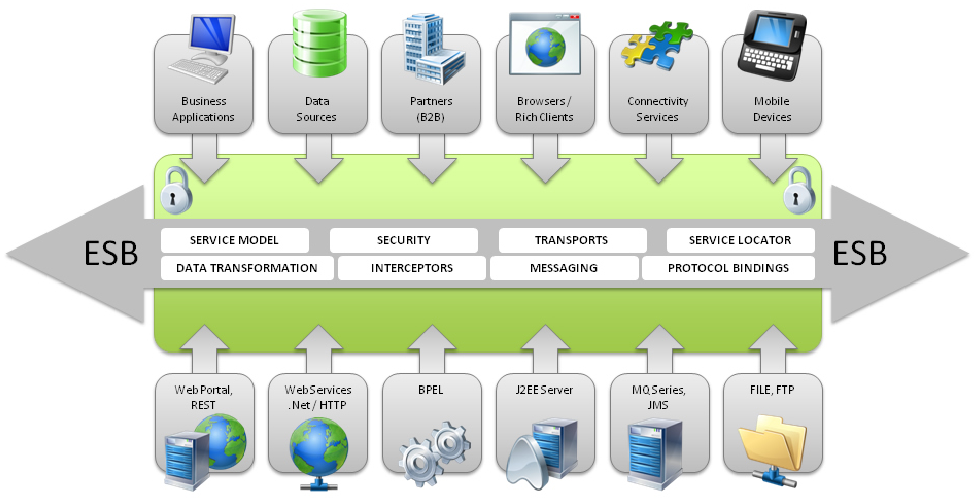
\includegraphics[width=0.8\textwidth]{esb_architecture}
    \caption{ESB arhitektura}
    \label{fig:esb-architecture}
\end{figure}

U ESB arhitekturi aplikacije su međusobno povezane preko ESB, umesto direktno jedna s drugom. ESB sadrži svu logiku za integraciju i interakciju između različitih servisa. 

\subsubsection{Funkcionalnosti}

Primarne funkcionlanosti ESB su:

\begin{itemize}
	\item Rutiranje poruka između servisa
	\item Monitoring i kontrola razmene poruka između servisa
	\item Upravljanje deployment-om i verzionisanjem servisa
	\item Upravljanje sa više instanci istog servisa
	\item Pružanje dodatnih usluga poput hendlovanja eventa, konvertovanje formata poruka, sekvenciranje poruka i event-ova, obrada izuzetaka, konverzije protokola itd. 
      \item Upravljanje transakcijama između više servisa
	\item Obezbeđivanje servisa od nedozvoljenog pristupa
\end{itemize}

\subsubsection{Implementacije}

Neke od popularnih implementacija ESB su: 
 
\begin{itemize}
	\item Jboss ESB
	\item Apache Servicemix
	\item Open ESB
	\item Mule ESB
	\item JBoss Fuse
\end{itemize}

\subsubsection{Prednosti i mane}

Neke od ključnih prednosti ESB arhitekture su: 

\begin{itemize}
	\item Nema dodatnog koda za integraciju servisa u sistem
	\item Podrška za transakcionu obradu podataka
	\item Podrška za redundantne instance servisa
	\item Mogućnost da se servisi projektuju tako da samo treba da ostvaruju neku funkcionalnost, bez razmišljanja o integraciji sa drugim servisima
\end{itemize}

Neke od mana ESB arhitekture su: 

\begin{itemize}
	\item Sporija komunikacija između servisa
	\item Single point of failure - u slučaju da ESB prestane sa radom, ceo sistem se zaustavlja
	\item Kompleksna konfiguracija sistema
	\item Otežano održavanje sistema
\end{itemize}


\chapter{Service mesh arhitektura}

Kao jedno od rešenja, pre svega infrastrukturnih, problema mikroservisnih sistema, smišljen je \textit{service mesh}. Service mesh (srp. servisna mreža, mreža servisa) je poseban infrastrukturni sloj. Konfigurabilan je, ima malu latentnost i dizajniran je tako da podnese intenzivnu interservisnu komunikaciju. Neke od rešenja koje donosi service mesh su: 

\begin{itemize}
	\item olakšano rutiranje
	\item jednostavnije postavljanje novih instanci na server
	\item jednostavna autorizacija i autentifikacija pri interservisnoj komunikaciji
	\item \textit{load balancing}-a (srp. raspoređivanje opterećenja - obrazac po kome se zahtevi raspoređuju ravnomerno svim dostupnim instancama servisa)
	\item enkripcija komunikacije
	\item \textit{circuit breaker} obrazac (srp. prekidač - obrazac kojim se omogućava servisima koji su oboreni ili zatrpani zahtevima, da se oporave)
\end{itemize}

Service mesh je alat koji pomaže u monitoringu, komunikaciji između servisa i kontrolisanju stanja sistema. To je zasebna infrastrukturna komponenta koja se sastoji iz dve ravni: 
\begin{itemize}
	\item ravan podataka (engl. \textit{data plane})
	\item ravan kontrole (engl. \textit{control plane})
\end{itemize}

Ravan podataka upravlja komunikacijom između instanci servisa. Kontrolna ravan generiše konfiguraciju i dostavlja je do svih instanci u ravni podataka. Korisnik se na kontrolnu ravan može povezati ili API-jem, terminalom ili grafičkim interfejsom. Pregled najvažnijih komponenti service mesh-a dati su na slici  \ref{fig:service-mesh-topology}. \newline

\begin{figure}[h]
    \centering
    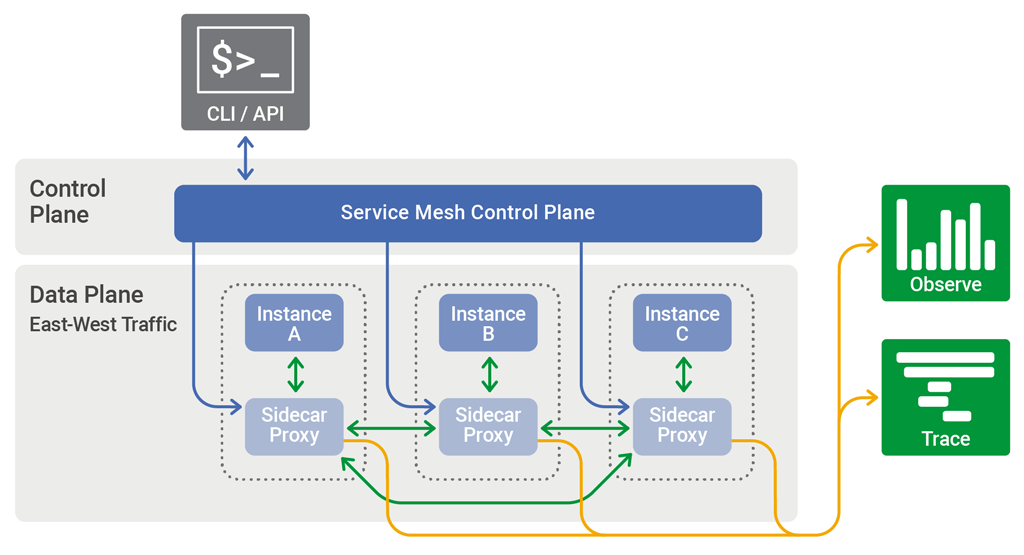
\includegraphics[width=\textwidth]{service-mesh-generic-topology}
    \caption{Service mesh topologija}
    \label{fig:service-mesh-topology}
\end{figure}

U ravni podataka svakoj od deploy-ovanih instanci servisa pridružen je i (jedan ili više) \textit{proxy} (srp. posrednik). Zajedno, instanca i njen proxy čine \textit{sidecar} (srp. prikolica) obrazac.  U sidecar obrascu se sve dodatne mogućnosti koje su potrebne servisu, dodaju u proxy-ju koji je zaseban kontejner koji se deploy-a uz aplikaciju. Ovaj obrazac omogućava da se dodaju nove funkcionalnosti bez izmene servisa. Na ovaj način se u service mesh-u dodaju funkcionalnosti poput monitoringa, logovanja, circuit breaker obrasca, load balancinga, enkripcije itd. Važno je napomenuti da bilo koji saobraćaj prvo prolazi kroz proxy, a zatim dolazi do servisa. Postoji još jedan obrazac koji se ređe koristi za deployment proxy-ja, a to je \textit{per-host} proxy. Kod per-host proxy-ja će svaki host imati svoj proxy. Jedan host može biti virutelna mašina, Kubernetes pod ili poseban server.  \newline

Na primer, ako jedan servis želi da komunicira s drugim servisom, taj zahtev presreće proxy servisa koji šalje zahtev. Proxy rutira zahtev do proxy-ja odredišta. Proxy odredišta presreće pristigli zahtev, pre nego što ga pošalje odredišnom servisu. Korišćenje proxy-ja olakšava da se sva svojstva nevezana za biznis logiku, a koja su zajednička za sve servise smeste u njega. Činjenica da saobraćaj prolazi kroz proxy-je omogućava da se beleži koji servisi međusobno komuniciraju, koliko traje komunikcija, i koliko je potebno da servisi odgovore na zahteve i koji je procenat uspešnosti i nespešnosti zahteva. \newline

Kontrolna ravan služi za centralizovano upravljanje service mesh-om. Bilo kakva promena ponašanja service mesh-a koja se primeni se najpre postavi na kontrolnu ravan i nakon toga kontrolna ravan primenjuje podešavanja na ravan podataka i na proksije. Na slici \ref{fig:service-mesh-topology} se takođe vidi da kontrolna ravan prikuplja i obrađuje telemetrijske podatke. Ovakva arhitektura servis mesha omogućava opcije poput monitoringa, circuit breakinga, canary releasing-a (tehnika kojom se nove promene postepeno uvode sve većem broju korisnika, kako bi se izbegli bug-ovi većih razmera), automatski TLS itd. \newline

Kontrolna ravan može da kontroliše i konfiguriše autorizaciju (koji servis može sa kojim da komunicira) i politiku rutiranja. Ovu konfiguraciju može da postavi korisnik, a onda će kontrolna ravan to proslediti ravni podataka. U ravni podataka se čita tekuća konfiguracija i komunicira se u skladu sa njom. \newline

Detaljnija arhitektura service mesh-a je data na slici \ref{fig:advanced-service-mesh-topology}.\newline

\begin{figure}[h]
    \centering
    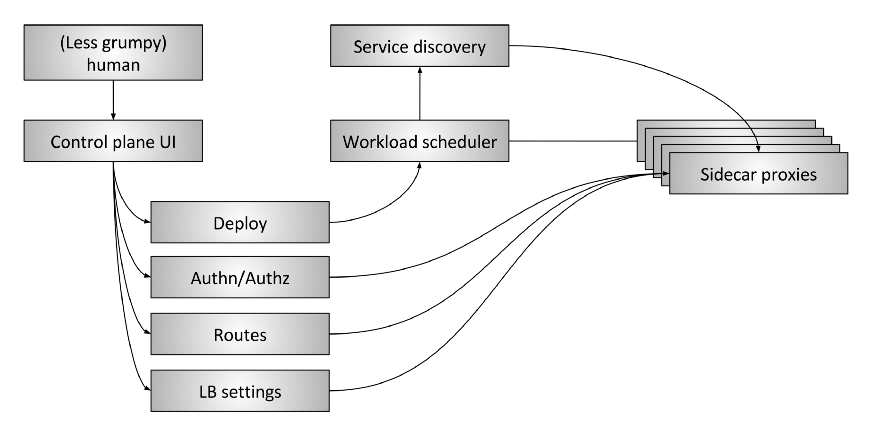
\includegraphics[width=\textwidth]{advanced-service-mesh-architecture}
    \caption{Detaljnija service mesh arhitektura}
    \label{fig:advanced-service-mesh-topology}
\end{figure}

Na slici \ref{fig:advanced-service-mesh-topology} su prikazane sledeće komponente service mesh sistema: 

\begin{itemize}
	\item čovek (engl. the human) - deo sistema koji donosi odluke visokog nivoa, vezane za rutiranje, autorizaciju itd. 
	\item UI ravni kontrole (engl. control plane UI) - čovek/korisnik interaguje sa korisničkim interfejsom kontrolne ravni (bilo da je to web UI, terminal itd). Kroz korisnički interfejs podešava se globalna konfiguracija sistema. Postavke deploymenta (blue/green i/ili preusmerenje saobraćaja), autentifikacija i autorizacija, tabela rutiranja, i postavke load balancinga (npr tajmauti, retries, circuit breakers itd).
	\item Workload scheduler - Servisi se postavljaju na servis mesh pomoću nekog scheduling sistema (npr. Nomad ili Kubernetes). Scheduling sistem je odgovoran za vezivanje servisa sa njegovim proxy-jem.
	\item Service discovery - Kako scheduler postavlja i gasi instance servisa, on to prijavljuje u service discovery sistem. 
\end{itemize}


\chapter{Svojstva service mesh arhitektura}

Sva svojstva service mesh arhitektura se mogu svrstati u jednu od tri kategorije:

\begin{enumerate}
	\item Upravljanje saobraćajem u sistemu
	\item Monitoring/nadgledanje sistema
	\item Bezbednost sistema
\end{enumerate}

Ova svojstva service mesh arhitektura čine ujedno su ujedno i njene prednosti. Korisnik ne mora da brine o tome kako da implementira sve ove funkcionalnosti, jer su one već implementirane za njega. On ima slobodu da podešava već postojeća svojstva i da time podiže stepen bezbednosti u sistemu, uključuje ili isključuje logovanje itd. 

\section{Upravljanje saobraćajem u sistemu}

Service mesh ima mogućnost da upravlja saobraćajem na mreži. Pri tom se uvode mnoga svojstva poput rutiranja, rate limiting (srp. ograničenje broja zahteva po servisu),  circuit breaking i tehnika mirroring. Kod service mesha se konfiguracija specificira na sedmom sloju OSI modela, aplikativnom sloju. Razdvajanje saobraćaja od infrastrukture, stavlja saobraćaj u nadležnost aplikacije i ljudi koji je održavaju. Vlasnici aplikacije i inženjeri najbolje razumeju potrebe aplikacije i prema tome mogu da podešavaju mrežne parametre kod aplikacije. \newline

\textbf{Pouzdana komunikacija}\newline

Service mesh osigurava pouzdanu mrežnu komunikaciju. Greške u komunikaciji se automatski rešavaju na transparentan način. U konfiguraciji se može navesti broj ponovnih pokušaja koji se može načiniti i timeout (vreme na koje se čeka na odgovor, nakon isteka tog vremena zahtev se smatra odbijenim). Slanje zahteva, čekanje i ponovno  Servis koji šalje zahtev svu komunikaciju prepušta proxy-ju. Taj proxy zatim šalje zahtev i čeka na odgovor. Ako odgovor ne dobije nakon timeout intervala, pokušava ponovo. Ako nakon zadatog broja pokušaja ne dobije odgovor, smatra da je servis nedostupan.  Na ovaj način se sva logika oko pouzdanosti prebacuje na proxy, dok se kod servisa ne treba menjati. \newline

\textbf{Circuit breaking}\newline

Ponovno slanje zahteva povećava pouzdanost sistema, međutim povećava i broj zahteva koje prima ciljni servis. Zbog ovoga će opterećenje ciljnog servisa biti veće i servis može postati nestabilan. Za rešavanje ovakvog problema uveo se circuit breaker. Ako je neki servis nedostupan on obično odgovara 503 zahtevom. U service meshu se može postaviti prag za broj ovakvih odgovora koji se mogu primiti. Nakon što se prag pređe, proxy izbacuje ovaj servis iz load balancer poola (load balancer pool - skup instanci servisa koje su dostupne). Novi zahtevi se neće rutirati ka "nezdravim" instancama. Najčešće se circuit breaker implementira tako što se navede maksimalni broj konkurentnih TCP konekcija i otvorenih HTTP zahteva. \newline

\textbf{Rate limiting}\newline

Rate limiting je povezan sa circuit breaking-om. Ta funkcionalnost omogućava da se ograniče zahtevi koji zadovoljavaju određeni kriterijum. To omogućava da se određeni zahtevi ne koriste previše. Ova funkcionalnost je slična otvorenim/javnim API-jevima koji kreću da se "guše" nakon što se pređe određen broj zahteva. Definisanjem rate limita zahteva da se definiše parametar koji se broji, maksimalna vrednost i vremenski prozor u kome se broji taj parametar. Broj zahteva se broji centralizovano tako da ceo sistem ima predstavu koliko zahteva je primljeno. Pažljiva konfiguracija rate limita će osigurati da svi korisnici imaju fer pristup servisu. \newline

\textbf{A/B testiranje}\newline

Upravljanje saobraćajem u service meshu omogućava A/B testiranje. Kada se testira web aplikacija, vlasnici aplikacije mogu da testiraju nove funkcionalnosti, tako što se deo saobraćaja rutira ka instancama servisa koje sadrže nove funkcionalnosti. Onda se može posmatrati telemetrije i da se proučava interakcija korisnika i funkcionalnosti. Iz te interakcije se mogu izvući zaključci da li se korisnicima više sviđa nova funkcionalnost ili stara, da li im se više sviđa jedna implementacija ili neka druga. Čest use-case za A/B testiranje mikroservisa je da se nove funkcionalnosti testiraju samo za ljude iz jednog regiona ili iz neke posebne grupe, ili da se neko ažuriranje proba na manjoj grupi korisnika, pre nego što se pusti svima. Uvek je moguće da se vrati prethodna verzija sistema ako se detektuje previše grešaka u novoj verziji servisa. Ako testiranje novih funkcionalnosti A/B testiranjem može negativno da utiče na sistem, preporučuje se da se koristi canary release.\newline

\textbf{Canary release}\newline

\begin{figure}[h]
    \centering
    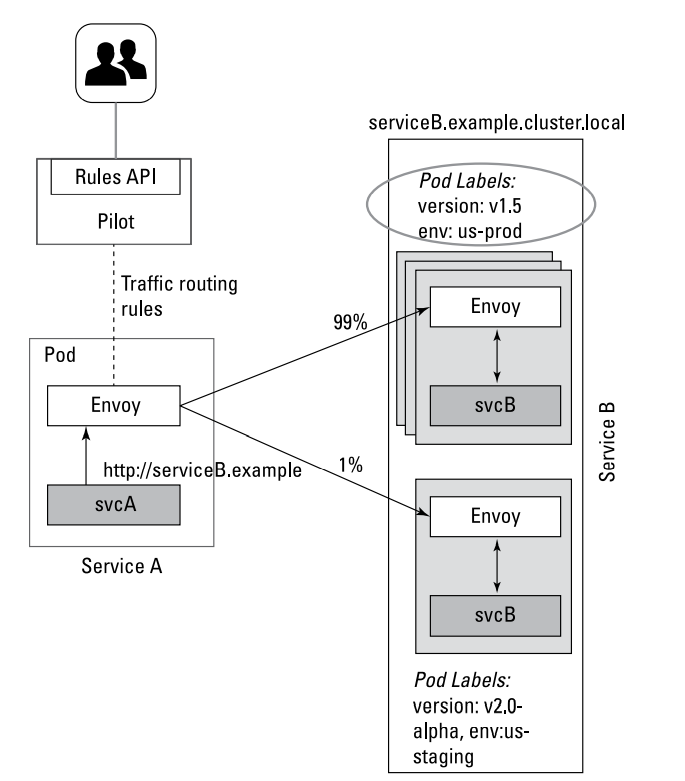
\includegraphics[width=0.5\textwidth]{canary_release_example}
    \caption{Primer Canary release-a}
    \label{fig:canary-release-example}
\end{figure}

Canary release je poseban slučaj A/B testiranja. Kod canary release se mnogo postepenije dešava zamena novih i starih replika. Početna faza kod canary release-a je tzv tamna faza. U ovoj fazi se novom servisu ne prosleđuje saobraćaj. Ako servis je servis "zdrav" vrlo mali procenat saobraćaja se rutira ka njemu (npr 1\%). Motri se na eventualne greške koje se mogu desiti. Sve dok je instanca zdrava, i dok nema grešaka, prosleđuje joj se sve više saobraćaja. Saobraćaj se prosleđuje postepeno, sve dok se 100\% ne bude usmereno ka novim instancama, a stare se postepeno isključuju. Na slici \ref{fig:canary-release-example} je dat primer canary release-a. U tom primeru se 99\% saobraćaja se usmerava ka verziji 1.5, a 1\% saobraćaja se usmerava ka 2.0 verziji. \newline

\textbf{Rutiranje}\newline

Rutiranje/upravljanje saobraćajem omogućava administratorima sistema da kontrolišu tok saobraćaja u aplikaciji. Pravilima rutiranja se određuje da li se može i gde pristigli saobraćaj proslediti na osnovu određenih osobina koji se prosleđuju u HTTP zaglavlju. Na primer, za komunikaciju između dva servisa je vrlo često potrebna neka vrsta autentikacije. Zato servis koji šalje zahtev stavlja u zaglavlje zahteva neki token koji će ga autentifikovati. Kada primajući proxy dobije zahtev, on vidi token za autentifikaciju, i ako je validan dopušta da zahtev stigne do instance. Ovim se eliminiše potreba da autentifikacija bude deo logike sistema, već se jednostavno navodi kao skup pravila u service meshu. Slično se može uraditi i sa lokacijom ili device-om koji šalje poruku. Npr deo saobraćaja se može rutirati, na osnovu lokacije/uređaja sa kojeg dolazi, ka određenom servisu.\newline

Na slici \ref{fig:routing-example} je dat prikaz rutiranja u service meshu. Na gornjoj polovini slike se svi zahtevi rutiraju iz servisa A ka servisu B. Canary release-om se uvodi novi servis za iPhone korisnike. Nakon promene politike rutiranja zahtevi se dele na one koji dolaze od Android uređaja i oni se i dalje rutiranju ka starim instancama servisa B, i zahteve koji dolaze od iPhone uređaja koji se rutiraju ka novoj instanci servisa B. \newline

\begin{figure}[h]
    \centering
    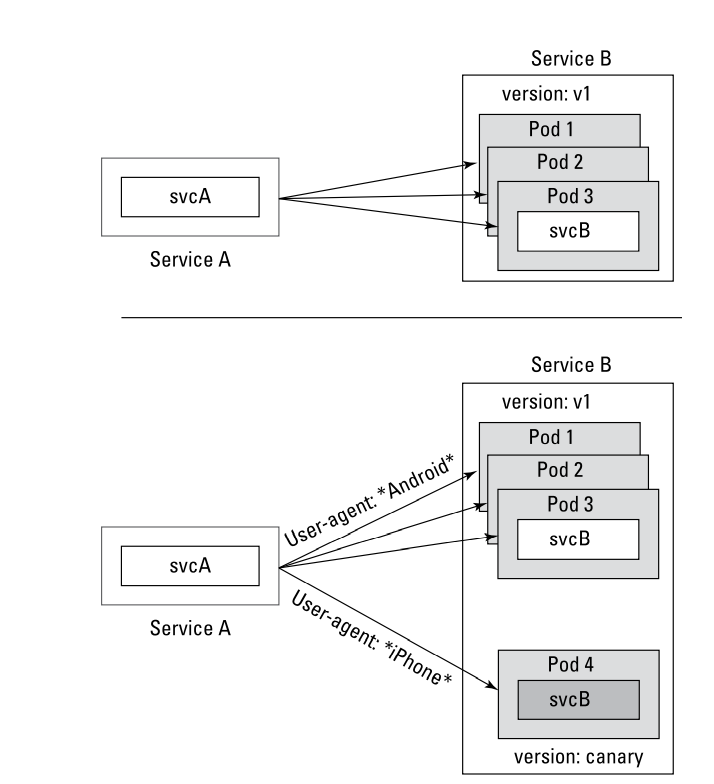
\includegraphics[width=0.7\textwidth]{routing_example}
    \caption{Primer rutiranja u service meshu}
    \label{fig:routing-example}
\end{figure} 

\textbf{Upravljanje spoljnim zahtevima}\newline

Service mesh, podrazumevano, ne dozvoljava spoljne konekcije ka servisima. Međutim, postoji način da se dozvole spoljne konekcije ka određenim URL-ovima. Kontrolisanje saobraćaja koji dolazi preko URL-ova pruža veći stepen fleksibilnosti od korišćenja firewall-a koji koriste IP adresu da filtriraju saobraćaj. Ovo je posledica toga da se IP adresa cloud aplikacije može lako menjati i nije fiksna. Jedan primer je mikroservisna aplikacija koja čita i piše u bazi. Baza je hostovana na javnom cloud-u van service mesha, bez statičke IP adrese. Izlazni saobraćaj mora da bude tako konfigurisan da mikroservisna aplikacija može da se poveže sa bazom koja je van mesha. Jedan pristup bi bio da se whitelist-uje ceo niz IP adresa koje koristi cloud provider. Ovakav pristup dovodi do mogućih bezbednosnih rizika. Sigurniji prilaz bi bio da se kreira poseban proxy - izlazni gateway (engl. egress gateway). Kroz ovaj gateway mora da prođe sav saobraćaj koji napušta service mesh. Korišćenje gateway-a pruža dodatnu kontrolu i može se koristiti Kubernetes za dodatno pooštravanje saobraćaja, tako da se onemogući da bilo koji izlazni saobraćaj, sem onog koji dolazi iz gateway-a, može da napusti klaster. \newline

\begin{figure}[h]
    \centering
    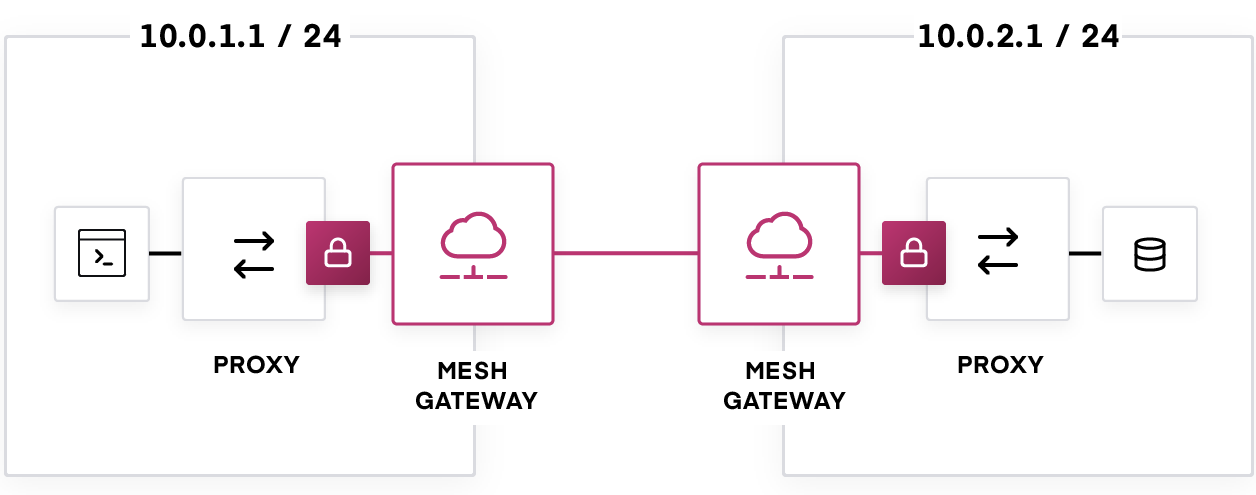
\includegraphics[width=0.7\textwidth]{egress_gateway_example}
    \caption{Primer komunikacije dva klastera preko izlaznog gatewaya}
    \label{fig:egress-gateway-example}
\end{figure} 

Na slici \ref{fig:egress-gateway-example} je dat primer komunikacije dva klastera preko izlaznog gateway-a. Na slici se vidi da se  aplikacija i njena baza nalaze na različitim mrežama. Ako aplikacija želi da komunicira sa bazom, mora da uputi zahtev na URL baze. Taj zahtev prolazi kroz proxy i na osnovu URL-a, proxy prosleđuje zahtev izlaznom gateway-u. Izlazni gateway zatim šalje zahtev na mrežu. Service mesh koji sadrži bazu prima zahtev preko svog izlaznog gateway-a. On se zatim rutira do odgovarajućeg proxy-ja i zatim stiže do servisa kom je bio namenjen. \newline

\section{Nadgledanje sistema}

\textbf{Monitoring}\newline

Mikroservisni sistem treba da uključuje i infrastrukturu za monitoring, koja će prikupljati informacije iz svih mikroservisa i omogućiti svima pristup tim informacijama. Ovo je neophodno da bi se motrilo na metrike velikog broja mikroservisa. Na osnovu ovih metrika se mogu implementirati alarmi ili da se rade dodatne analiza na osnovu ovih metrika. Proxy-ji u ravni podataka, mogu da mere osnovne informacije o mrežnom saobraćaju, kao što su latentnost i propusnost. Moguće je pored ovih informacija izvući još neke dodatne. Service mesh može da razume protokol i da ga tumači. Npr, HTTP protokol ima neki definisan statusni kod koji omogućava service mesh-u da "/ shvati "/ da li je zahtev bio uspešan ili ne. Na ovom osnovu, service mesh može da meri procenat uspešnosti i neuspešnosti zahteva.  Monitoring na nivou service mesh-a ima sledeće prednosti: 

\begin{itemize}
	\item Nema uticaja na kod mikroservisa. Metrike se mere samo u proxy-ju, tako da će svi mikroservisi meriti iste metrike, bez obzira u kom programskom jeziku su pisani ili koji framework koriste.
	\item Metrike daju na uvid stanje mikroservisa. Metrike pokazuju performanse i pouzdanost servisa, koje su korisne krajnjem korisniku i administratoru sistema. Ove metrike su dovoljne da se osigura očekivani kvalitet i pouzdanost servisa. 
\end{itemize}

Metrike koje pruža service mesh su dovoljne za održavanje mikroservisnog sistema. Ali za dublju analizu uzorka problema, potrebne su dodatne metrike koje dolaze iz servisa. U tom slučaju, service mesh takođe može biti od pomoći jer pruža standardizovano okruženje za monitoring, koje service mesh već koristi za svoje metrike. \newline

\textbf{Distribuirano trasiranje}\newline

Trasiranje rešava čest problem u mikroservisnim sistemima. Zahtev ka mikroservisu može za posledicu imati jedan ili više zahteva ka drugim servisima. Trasiranje omogućava praćenje ovakvih zahteva, time olakšavajući nalaženje srži nekog problema. Proxy-ji presreću svaki od zahteva. Međutim da bi bilo moguće raditi trasiranje, treba zaključiti koji zahtev je dolazni, a koji izlazni zahtev. Ovo se obično radi unutar servisa. Obično savaki od servisa ima nekakav jedinstveni ID u sebi, i ova informacija se zatim prosleđuje svim zahtevima koji nastaju od njega. Podaci o svakom zahtevu se  zatim čuvaju u service meshu. Jedinstveni ID nije samo koristan za trasiranje, već se koristi i pri logovanju i može biti jako koristan za praćenje zahteva u servisima. Trasiranje se obično koristi u vrlo specifičnim situacijama, gde je vrlo složena komunikacija između servisa. U većini slučajeva se analiza grešaka može izvršiti samo gledanjem u jedan od servisa, smatrajući ostale crnim kutijama. Podacima prikupljenim trasiranjem se mogu kreirati grafovi zavisnosti. koji ukazuju na to koji servisi međusobno komuniciraju. \newline

\textbf{Logovanje}\newline

Logovanje je još jedan način da se stekne uvid u funkcionisanje mikroservisnog sistema. Service mesh prikuplja informacije o mrežnoj komunikaciji. Te informacije može da piše u log fajl. Pristupni logovi koji sadrže unose za HTTP pristup su važni izvor informacija o radu web aplikacije. Često se log fajlovi koriste za analizu grešaka u mikroservisnom sistemu. Da bi se to uradilo, log fajlovi moraju da imaju detaljne informacije. Mikroservisi moraju sami da loguju tu informaciju. Slično kao kod trasiranja i ovo zahteva promenu načina funkcionisanja servisa. Automatski logovi service mesh-a daju samo informacije o komunikaciji, i primljenim porukama što obično nije od značaja. Prednost Logovanje kod service mesh-eva je ta da programeri ne moraju uopšte da se bave logovanjem. Logovi su uniformni bez obzira na tehnologiju i način logovanja. Čak i ovakvi logovi mogu pomoći prilikom traženja grešaka. \newline
 
\section{Bezbednost sistema}

Bezbednost service mesh sistema uključuje slučajeve kao što su autorizacija i autentifikacija. \newline

\textbf{mTLS autentikacija}\newline

\textit{Mutual authentication} (skr. mTLS) je protokol kojim se simultano autentifikuju dve strane u komunikaciji. Ovakav protokol je namenjen prenosu osetljivih podataka kroz mrežu. Interservisna komunikacija se u service meshu odvija preko proxy-jeva. Proxy-ji mogu da generišu mTLS tunele između servisa, i svaki servis će imati svoj jedinstveni sertifikat koji garantuje identitet. Sertifikatima se upravlja u centralizovanoj komponenti koja je takođe odgovorna za rotaciju sertifikata. Enkripcija je vrši na sedmom nivou OSI, što znači da se enkriptuje sadržaj, a ne saobraćaj. 
Postoje dva tipa enkripcije: 

\begin{itemize}
	\item restriktivni - kod ovog tipa enkripcije se servis konfiguriše da ne prihvata neenkriptovani saobraćaj
	\item  permisivni - kod ovog tipa enkripcije servis prihvata i neenkriptovani saobraćaj po potrebi
\end{itemize}

\textbf{Autorizacija}\newline

Autorizacija je analogna mikrosegmentaciji na sedmom nivou OSI. Mikro-segmentacija se sprovodi po principu nultog poverenja. Mikro-segmentacija znači da nijedan saobraćaj koji nema eksplicitinu dozvolu neće biti propušten. Svakom dolaznom zahtevu se ispituje header u potrazi za potrebnom dozvolom. U service mesh sistemima, autorizacija se pruža na nivou imenskog prostora, na servisnom nivou i na nivou pojednih metoda (tzv. endpointa). \newline

Na slici \ref{fig:authorization-architecture} je dat primer autorizacije u service mesh sistemu. Kada proxy primi zahtev on čita trenutnu autorizacionu konfiguraciju i vidi da li taj zahtev dolazi od izvora koji ima pristup. Na osnovu toga se zahtev prihvata ili odbija. 

\begin{figure}[h]
    \centering
    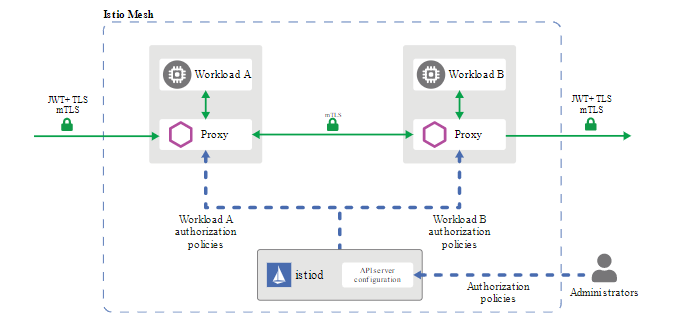
\includegraphics[width=0.7\textwidth]{authorization_architecture}
    \caption{Primer autorizacije u service mesh sistemu}
    \label{fig:authorization-architecture}
\end{figure} 

\chapter{Implementacije service mesh sloja}

U nastavku će biti opisan Consul kao primer implementacije service mesh infrastrukturnog sloja. Consul je Hashicorp-ova implementacija service mesha. Najčešće se upotrebljava za otkrivanje i konfigurisanje različitih servisa koji su deo sistema. Pisan je u Golangu. Consul se na server može postavljati na samoj mašini kao standalone aplikacija ili mnogo češće kao Docker kontejner ili kao pod u Kubernetes klasteru. 

\section{Druge implementacije service mesh sloja}

\subsection{Istio}

Istio je jedan od najpopularnijih open source service mesh rešenja, koje koriste IBM, Google i Red Hat. Istio je jedna od prvih service mesh platformi koja koristi Envoy kao proxy. Arhitektura Istio service mesh-a je klasična podela na centralnu kontrolnu ravan i distribuiranu ravan podataka sa pridruženim mikroservisima. Na slici \ref{fig:istio-architecture} je data arhitektura Istio service mesh rešenja. \newline

\begin{figure}[h]
    \centering
    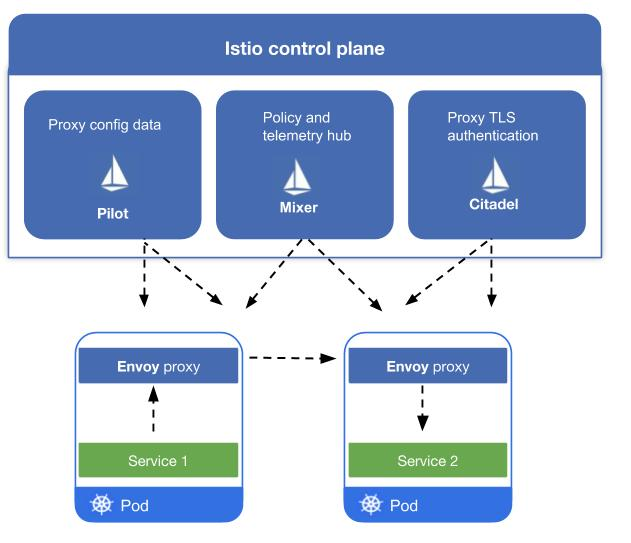
\includegraphics[width=0.5\textwidth]{istio_architecture}
    \caption{Istio service mesh arhitektura}
    \label{fig:istio-architecture}
\end{figure}

Istio pruža tri ključne prednosti mikroservisnim arhitekturama: 

\begin{itemize}
	\item Upravljanje saobraćajem - Istio pojednostavljuje konfigurisanje opcija poput circuit breaking, timeout, retries itd. Takođe olakšava implementaciju canary release, A/B testiranja itd. 
	\item Bezbednost - Istio pruža ugrađenu podršku za međuservisnu komunikaciju. Pruža bezbedne komunikacione kanale, upravlja autorizacijom i autentifikacijom i enkripcijom poruka. Takođe omogućava specifikaciju pravila, koji servis sa kojim može da komunicira. 
	\item Monitoring - Istio proxy presreće sav dolazni i odlazni saobraćaj. Time ima uvid u trenutno stanje servisa. Istio pruža opcije za trasiranje saobraćaja, monitoring, i logovanje da bi se stekao uvid u runtime performanse sistema. 
\end{itemize}

\subsection{Linkerd 2.x}

Linkerd 2.x je open source service mesh platforma koja ima ekskluzivnu podršku za Kubernetes. Ima 3 komponente:

\begin{enumerate}
	\item CLI i UI
	\item  control plane
	\item  data plane
\end{enumerate}

Komponente Linkerd 2.x sistema su dati na slici \ref{fig:linkerd-architecture}. Sve komponente kontrolne ravni se instaliraju kao Kubernetes deployment unutar linkerd namespace-a. Kontrolnoj ravni se može pristupati preko CLI i web interfejsom, i one koriste public api komponentu kontrolera. Destination komponenta čuva i komunicira informacije o rutiranju proksijima. Injector komponenta dodaje proxy svaki put kada se novi pod deploy-a na sistem. Identity komponenta čuva sertifikate koji se koriste pri komunikaciji između servisa. Tap komponenta prima zahteve od CLI i web UI, o praćenju zahteva u realnom vremenu.\newline

Svakom servisu u sistemu pridružen je proxy. Linkerd koristi sopstvenu implementaciju proxy-ja, umesto Envoy proxy-ja koji koriste sve ostale service mesh implementacije. Linkerd ima podršku za rutiranje, za sigurnu komunikaciju i monitoring, kao Istio. 

\begin{figure}[h]
    \centering
    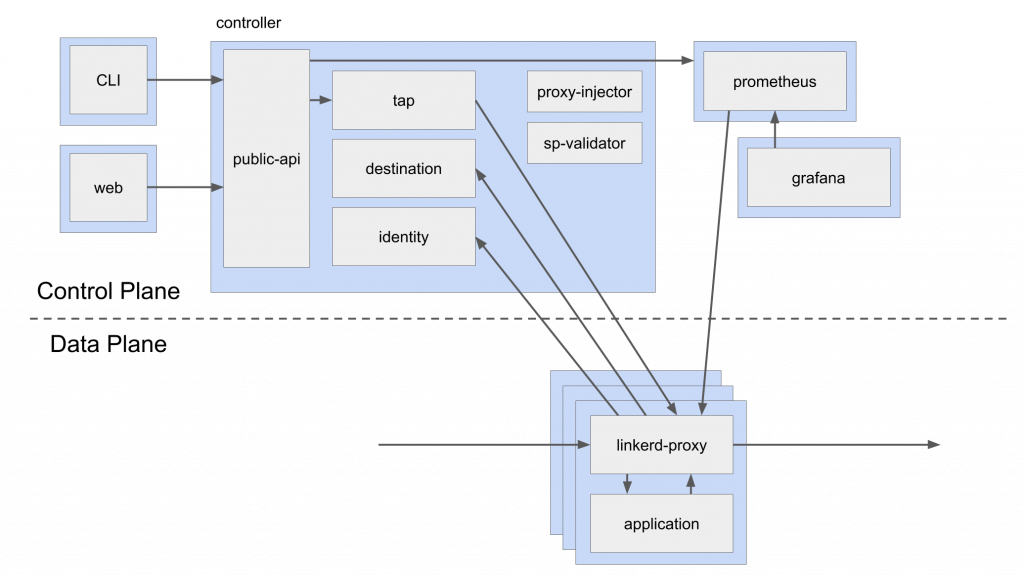
\includegraphics[width=0.7\textwidth]{linkerd_architecture}
    \caption{Linkerd service mesh arhitektura}
    \label{fig:linkerd-architecture}
\end{figure}


\section{Arhitektura i funkcionalnosti Consula}

Srž Consul sistema je proces Consul agent. Agent čuva informacije o članstvu u service meshu, može da registruje servise, da vrši health checking, odgovara na upite, daje informacije o sistemu itd. Consul agent može da bude deploy-ovan u dva različita moda, \textit{klijent} i \textit{server}: 

\begin{itemize}
	\item server - Consul agent koji je u server modu i služi da održava stanje klastera
	\item klijent - Consul agent kojih ima mnogo više u sistemu (nalaze se u svakom čvoru sistema) i služe da komuniciraju sa serverima, pribavljaju konfiguraciju i komuniciraju je do proxy-ja. 
\end{itemize}

Svaki od Consul agenta u sebi ima informacije o : 

\begin{itemize}
	\item Ime čvora (engl. \textit{node name}) - ime hosta na kom se agent nalazi
	\item Ime datacentra (engl. \textit{datacenter}) - ime datacentra za koji je Consul konfigurisan. Svaki čvor se morati odazivati svom datacentru. 
	\item Server - svaki agent ima indikator da li se izvršava u klijent ili server modu. Čvorovi koji se izvršavaju u server modu učestvuju u kvorumima konzenzusa, čuvanju informacija o stanju klastera. 
	\item Adresu klijenta - adresa koju agent koristi za interfejse klijenta. Uključuje portove za HTTP, RPC i DNS. 
	\item Adresu klastera - adresa i skup portova koja se koristi za komunikaciju između Consul agenta u klasteru. Adresa mora da bude dostupna za sve ostale agente u klasteru.
\end{itemize}

Consul ima podršku za Envoy implementaciju sidecar proxy-ja.  Ovi proxy-ji kontrolišu sav saobraćaj koji ulazi i izlazi iz servisa. \newline

Na slici \ref{fig:consul-architecture} je dat prikaz arhitekture Consul service mesha. Detaljnija arhitektura Consul service mesha na kojoj je prikazana i interakcija servisa sa komponentama Consul sistema data je na slici \ref{fig:detailed-consul-architecture}. \newline

\begin{figure}[h]
    \centering
    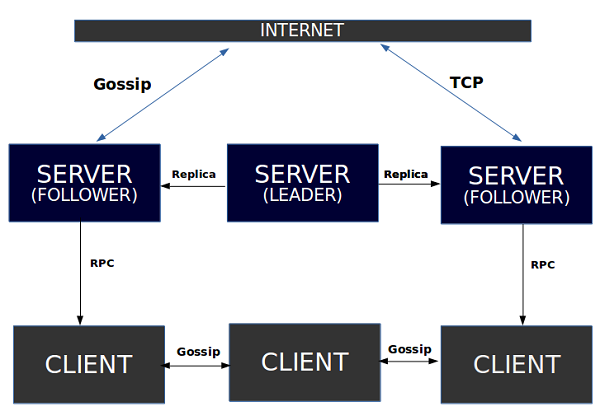
\includegraphics[width=0.9\textwidth]{consul_architecture.jpg}
    \caption{Primer arhitekture Consul service mesha}
    \label{fig:consul-architecture}
\end{figure} 

\begin{figure}[h]
    \centering
    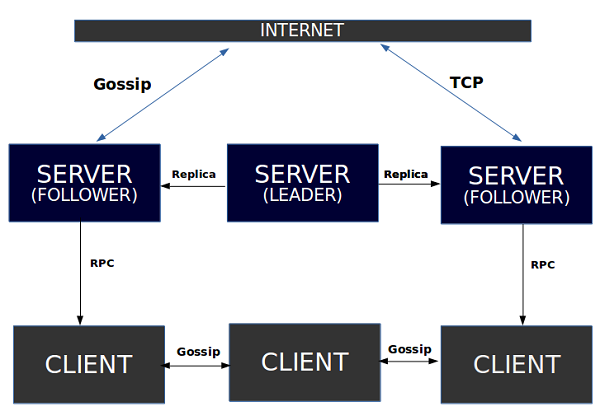
\includegraphics[width=0.9\textwidth]{consul_architecture}
    \caption{Detaljna arhitektura Consul service mesh}
    \label{fig:detailed-consul-architecture}
\end{figure} 

Na slici \ref{fig:consul-architecture} se vide da postoje tri Consul agenta koji se nalaze u serverskom modu (u opštem slučaju ih može biti n). Raft algoritmom (raft - srp. splav), se od ova tri agenta bira jedan koji će biti lider i ostali koji će biti pratioci. Pratioci treba da prate odluke koje donosi lider. Sva tri servisa su međusobno povezana radi dalje komunikacije. Svaki od servera interaguje sa svojim klijentom putem RPC protokola. Komunikacija između klijenta se odvija tzv Gossip protokolom. \newline

\textbf{Raft algoritam}\newline

Raft algoritam služi za ostvarivanje konsenzusa. Raft klaster se sastoji od  nekoliko servera (obično neparan broj). Server može biti u nekom od tri stanja: \textit{Lider}, \textit{Pratilac} ili \textit{Kandidat}. Kada je sistem u stabilnom stanju postoji samo jedan lider i svi ostali su pratioci. Pratioci se nalaze u pasivnom stanju, tj. nemaju nikakve svoje zahteve već samo odgovaraju na zahteve lidera i eventualnih pratilaca. Na slici \ref{fig:raft-algorithms} se nalazi dijagram koji prikazuje način na funkcionisanja raft algoritma. \newline 

\begin{figure}[h]
    \centering
    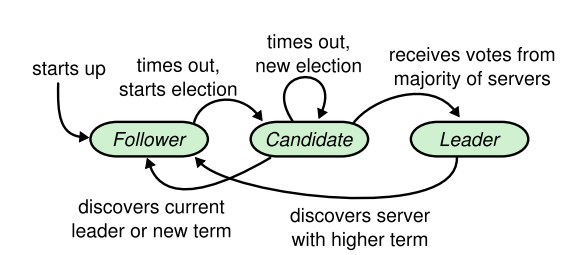
\includegraphics[width=0.9\textwidth]{raft_algorithm}
    \caption{Raft algoritam}
    \label{fig:raft-algorithms}
\end{figure} 

Neko od pratioca započinje izbor novog lidera, nakon timeouta. Pratioc menja stanje u kandidata za lidera. Ako u sistemu, već postoji lider, kandidat ga detektuje i menja stanje u pratioc. U suprotnom, sve dok neko od kandidata ne dobije većinu glasova od ostatka, izbor se nastavlja. \newline

\textbf{Key value store}\newline

Od verzije Consula 0.7.1, postoji podrška za key-value store. Ovoj store se može pristupati preko komandne linije ili preko Consul UI, i podržava se dodavanje, ažuriranje, prikaz i brisanje podataka iz nje. Struktura koju čuva key value store je data na slici \ref{kv-ds}. \newline

\begin{figure}

\begin{verbatim}
type KVPair struct {
   	Key string
   	CreateIndex uint64
   	ModifyIndex uint64
   	LockIndex uint64
   	Flags uint64
   	Value []byte
   	Session string
}
\end{verbatim}
    \caption{Key-value struktura podataka}
    \label{kv-ds}
\end{figure}

Key parametar sa slike \ref{kv-ds} je ključ za koji treba zapamtiti neku vrednost. CreateIndex je vrednost indeksa koja je dodeljena kada je podatak prvi put upisan u KV store. ModifyIndex je broj indeksa koji je dodeljen u trenutku kada je unos ažuriran poslednji put. LockIndex čuva broj puta puta koliko je lock stavljen nad tim unosom. Flags polje može da se koristi od strane aplikacije za postavljanje različitih vrednosti koje se mogu i ne morjau koristiti kao flegovi. Value je vrednost koja se pamti, enkodirana kao base64 blob. Session polje daje informaciju o sesiji koja poseduje lock na unos. \newline

Protokol kojim se komunicira između klijenata u Consul klasteru, je Gossip (srp. tračarenje) protokol. Kod ovog protokola vesti se prenose od čvora do čvora. Ovim protokolom se reguliše članstvo u klasteru i komunikacija između klijenata u klasteru. U okviru Consula, formiraju se dva pool-a, LAN i WAN poolovi. Svaki Consul datacentar ima svoj LAN pool u kome se nalaze svi serveri i klijenti koji mu pripadaju. Ovaj LAN pool olakšava klijentima da detektuju servere i smanjuje količinu potrebne konfiguracije. Ako dođe do pada nekog od servera (ili bilo kog drugog čvora) ova informacija se jako brzo može proširiti po celom klasteru. Takođe LAN pool-ovi omogućavaju brz i jednostavan broadcast poruka. \newline

WAN pool je jedan, i globalno jedinstven, i svi serveri iz svih datacentara mu pripadaju. Prisustvo servera u WAN pool-u im omogućava da izvršavaju zahteve koji se prostiru kroz više datacentara. \newline

Neke od funkcionalnosti koje nudi Consul su service discovery, bezbednost, telemetrija i monitoring, load balancing, health checking, rutiranje. \newline

\textbf{Service discovery}\newline

Jedna od najvažnijih funkcionalnosti service mesha je otkrivanje servisa. Consul se lako može deploy-ovati na svim postojećim cloud arhitekturama ili na bilo kom kontejneru, virtuelnoj mašini i na pravom serveru. Bez obzira da li se nalazi na istoj mreži ili ne, sa ostalim servisima, on može da ih otkrije. Ovim je postignuta velika fleksibilnost u sistemu, jer način i pozicija deploymenta ne zavisi od toga da li će servis biti otkriven, što pojednostavljuje service discovery funkcionalnost i omogućava projektantima sistema da koriste samo jedno service discovery rešenje umesto više njih. \newline

\textbf{Bezbednost}\newline

Za implementaciju bezbednosti Consul nudi više rešenja koja se mogu koristiti. Jedno od njih je Consul Connect koji pomaže u uspostavljanju zero-trust politike u komunikaciji. Zero-trust politika komunikacije se ovde uspostavlja preko mTLS konekcije između servisa. Ovako osigurane konekcije mogu da se prostiru na više datacentara i platformi. Consul Intentions je jedan od alata kojim se definiše 	kontrola pristupa preko Connecta. Intentions služi da definiše koji servisi smeju, a koji ne, da uspostave konekciju. Najčešće proxy osigurava sprovođenje politike zadate u Intentionsu. Consul ACLs su access liste kojima se obezbeđuju individualni endpointi, CLI ili GUI.  \newline

\textbf{Telemetrija i monitoring}\newline

Consul prikuplja različite metrike dok program radi. Ove metrike se najčešće prikupljaju na intervalu od 10s i čuvaju se do 1 minuta. Zatim se ove metrike strimuju do dela sistema zaduženog za čuvanje i obradu metrika, tzv. metrics store. Telemetrija i montiroing celog klastera, tako i pojedinih servisa pruža uvid u health celog klastera, i u unutrašnje funkcionisanje svakog od servisa.  \newline

\textbf{Load balancing}\newline

Consul automatski balansira opterećenje između zdravih instanci servisa u sistemu. Consul takođe omogućava publisher-subscriber mehanizam. Kada se servis registruje na sistem pri deploymentu, middleware može da se subscribuje na ovakve eventove (promena servisa) i da izvrši automatsku rekonfiguraciju. Ovo je korisno kada u sistemu postoji NGINX, F5 itd. \newline

\textbf{Health checking}\newline

Consul periodično vrši health checking u svim klasterima, da odvoji zdrave instance servisa od onih koje nisu funkcionalne. Zbog toga uvek postoji jasan pregled zdravih i nezdravih instanci servisa. \newline

\textbf{Rutiranje}\newline

Consul može da rutira saobraćaj na sedmom OSI nivou, korišćenjem proxy-ja i Consul Connecta. Sa mogućnošću rutiranja u Consulu, moguće je implementirati A/B testiranje, Canary release, itd. \newline

\section{Implementacija }

U narednoj glavi biće demonstrirane funkcionalnosti Consul service mesha, preko sample aplikacije koja se može besplatno preuzeti sa sajta zvanične Consul dokumentacije.  Biće demonstrirane funkcionalnosti poput health checking-a, service discovery-ja, rutiranja, load balancinga, canary release.  \newline

\textbf{Struktura aplikacije}\newline

Za demonstraciju funkcionalnosti Consul service mesha biće korišćene aplikacije koje su kontejnerizovane i deploy-ovane uz pomoć Dockera. Biće deploy-ovana dva servisa i Consul agent u server modu. Servisi se kreiraju iz nicholasjackson/fake-service:v0.4.1 image-a.  Ovim image-om se deploya servis koji vraća određenu poruku kada se pogodi GET HTTP zahtevom. Uz svaku od aplikacija, biće deploy-ovan i consul-envoy proxy, koji zajedno sa aplikacijom implementira Consul sidecar pattern. \newline

Aplikacija kojom će se demonstrirati funkcionalnosti Consula se sastoji iz dva servisa, web servis i payments servis i svaki od servisa ima svoj proxy. Uz servise biće deploy-ovan i jedan Consul agent u serverskom režimu rada. Strukturni dijagram aplikacije dat je na slici \ref{fig:structure-diagram}.\newline

\begin{figure}[h]
    \centering
    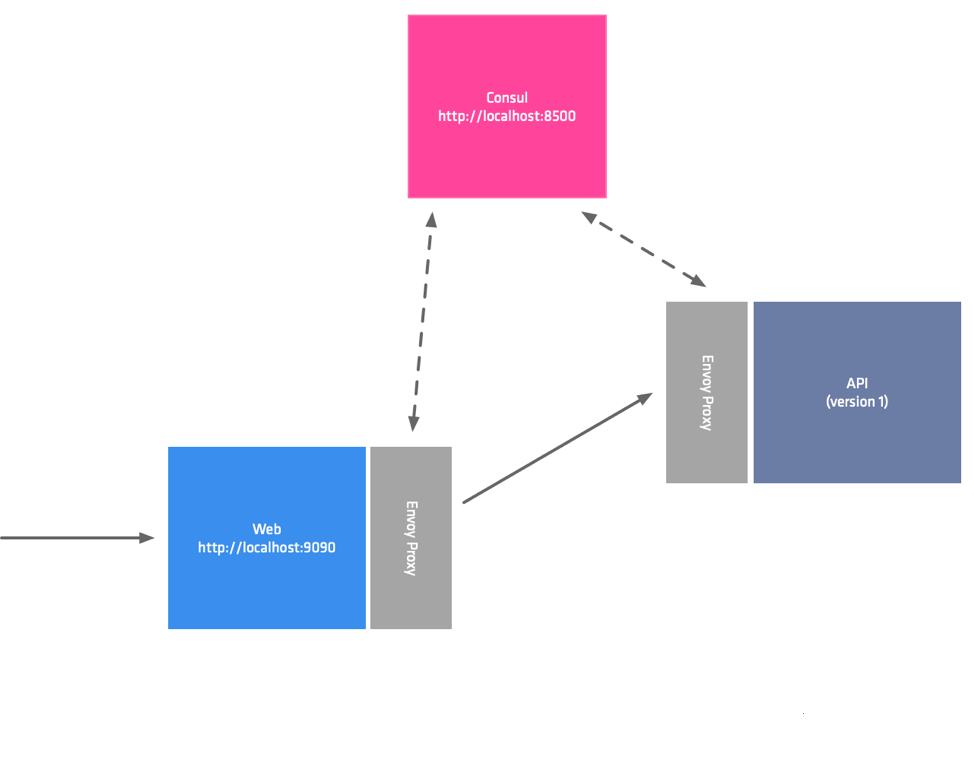
\includegraphics[width=0.9\textwidth]{app_structure_diagram_start}
    \caption{Strukturni dijagram aplikacije}
    \label{fig:structure-diagram}
\end{figure} 

Web servis je kao API gateway aplikacije i on prosleđuje pozive ka payment servisima.  Kada web servis primi zahtev on ga prosleđuje tzv. upstream (srp. uzvodnim) servisima, tj rutira zahtev prema servisu koji ga obrađuje. U ovom slučaju to će biti payment servis. \newline

\textbf{Demonstracija karakteristika Consula}\newline

Consul, web i payment servis kao i odgovorajaući proxy-ji će biti kreirani jednim docker-compose fajlom. Svaki od elemenata će činiti zaseban kontejner i svi kontejneri će biti deo iste mreže, kako bi jedno drugom bili vidljivi. Na listingu \ref{dc-consul} je dat deo docker-compose fajla koji se odnosi na Consul i njegov deployment. \newline

\begin{lstlisting}[
    basicstyle=\small,
    caption = Deo docker-compose fajla koji se odnosi na Consul, 
   label = dc-consul
]
  consul:
    image: consul:1.6.0
    command: ["consul","agent","-config-file=/config/consul-single-dc.hcl","-config-dir=/config"]
    volumes:
      - "../consul_config:/config"
    ports:
      - 8500:8500
    networks:
      vpcbr:
        ipv4_address: 10.5.0.2
\end{lstlisting}

U listingu \ref{dc-consul} se jasno vidi da se koristi image consul:1.6.0, da se izvršava na portu 8500 i da pripada vpcbr mreži i da je u okviru te mreže njegova adresa 10.5.0.2. Takođe komanda koja se upućuje kontejneru pri podizanju je \texttt{consul agent -config-file=/config/consul-single-dc.hcl -config-dir=/config}, kojom se navodi da Consul čuva podatke u /config direktorijumu i da je fajl u kom se nalazi konfiguracija Consula consul-single-dc.hcl. U ovom dokumentu se nalaze podešavanja kojima se Consulu kaže kako je ime datacentra, u kom modu se izvršava, da li je dozvoljen Consul connect, na kom mrežnom interfejsu se izvršava, koji je log level itd. Consul konfiguracioni fajl je dat na listingu \ref{hcl}. \newline

\begin{lstlisting}[
    basicstyle=\small,
    caption = Konfiguracioni fajl za Consul server, 
   label = hcl
]
data_dir = "/tmp/"
log_level = "DEBUG"
datacenter = "dc1"
server = true
bootstrap_expect = 1
ui = true
bind_addr = "0.0.0.0"
client_addr = "0.0.0.0"
ports {
  grpc = 8502
}
connect {
  enabled = true
}
advertise_addr = "10.5.0.2"
enable_central_service_config = true
\end{lstlisting}


\begin{lstlisting}[
    basicstyle=\small,
    caption = Deo docker-compose fajla koji se odnosi na web servis i njegov proxy, 
   label = web-service-dc
]
web:
    image: nicholasjackson/fake-service:v0.4.1
    environment:
      LISTEN_ADDR: 0.0.0.0:9090
      UPSTREAM_URIS: http://localhost:9091
      NAME: web
      MESSAGE: "Hello World"
      HTTP_CLIENT_KEEP_ALIVES: "false"
    networks:
      vpcbr:
        ipv4_address: 10.5.0.3
    ports:
      - 9090:9090
  web_envoy:
    image: nicholasjackson/consul-envoy:v1.6.0-v0.10.0
    environment:
      CONSUL_HTTP_ADDR: 10.5.0.2:8500
      CONSUL_GRPC_ADDR: 10.5.0.2:8502
      SERVICE_CONFIG: /config/web_v1.hcl
    volumes:
      - "./service_config:/config"
      - "./central_config:/central_config"
    command: ["consul", "connect", "envoy","-sidecar-for", "web-v1","--","-l","debug"]
    network_mode: "service:web"
\end{lstlisting}

Deo docker-compose fajla koji se odnosi na web servis i njegov proxy dat je na listingu \ref{web-service-dc}. Image koji se koristi za ovaj kontejner je \texttt{nicholasjackson/fake-service:v0.4.1}. Ovom servisu je potrebno preko promenljivih okruženja proslediti adresu na kojoj sluša, eventualne upstream servise kojima će dalje da prosleđuje zahtev, koja mu je poruka i u koja mu je adresa u okviru mreže vpcbr. \newline

Web proxy se kreira iz image-a \texttt{nicholasjackson/consul-envoy:v1.6.0-v0.10.0}, i prosleđuju mu se adrese preko kojih može da se obrati Consul serveru i putanja do konfiguracionog fajla. Naredba kojom se startuje web proxy kontejner je \texttt{consul connect envoy -sidecar-for web-v1 -- -l debug}, kojom se navodi da je taj proxy vezan za web servis. Na listingu \ref{web-service-conf} je prikazan konfiguracioni fajl za web servis proxy. \newline

\begin{center}
\begin{lstlisting}[
    basicstyle=\small,
    caption = Konfiguracioni fajl za web proxy, 
   label = web-service-conf
]
service {
  name = "web"
  id = "web-v1"
  address = "10.5.0.3"
  port = 9090
  connect { 
    sidecar_service {
      port = 20000
      check {
        name = "Connect Envoy Sidecar"
        tcp = "10.5.0.3:20000"
        interval ="10s"
      }
      proxy {
        upstreams {
          destination_name = "payments"
          local_bind_address = "127.0.0.1"
          local_bind_port = 9091
        }
      }
    }  
  }
}
\end{lstlisting}
\end{center}





Deo docker-compose fajla koji se odnosi na payments servis i njegov proxy dat je na listingu \ref{payments-service-dc}. Image koji se koristi za ovaj kontejner je nicholasjackson/fake-service:v0.4.1, kao u prethodnom slučaju. Ovom servisu je potrebno preko promenljivih okruženja proslediti adresu na kojoj sluša i poruku kojom odgovara na zahtev kao i adresu u okviru vpcbr mreže. \newline

\begin{lstlisting}[
    basicstyle=\small,
    caption = Deo docker-compose fajla koji se odnosi na payments servis i njegov proxy, 
   label = payments-service-dc
]
payments_v1:
    image: nicholasjackson/fake-service:v0.4.1
    environment:
      LISTEN_ADDR: localhost:9090
      NAME: payments-v1
      MESSAGE: "PAYMENTS V1"
    networks:
      vpcbr:
        ipv4_address: 10.5.0.4
  payments_proxy_v1:
    image: nicholasjackson/consul-envoy:v1.6.0-v0.10.0
    environment:
      CONSUL_HTTP_ADDR: 10.5.0.2:8500
      CONSUL_GRPC_ADDR: 10.5.0.2:8502
      SERVICE_CONFIG: /config/payments_v1.hcl
      #      CENTRAL_CONFIG: "/central_config/api_service_defaults.hcl"
    volumes:
      - "./service_config:/config"
      - "./central_config:/central_config"
    command: ["consul", "connect", "envoy","-sidecar-for", "payments-v1"]
    network_mode: "service:payments_v1"
\end{lstlisting}

Payments proxy se kreira iz image-a nicholasjackson/consul-envoy:v1.6.0-v0.10.0, i prosleđuju mu se adrese preko kojih može da se obrati Consul serveru i putanja do konfiguracionog fajla. Naredba kojom se startuje payments proxy kontejner je \texttt{consul connect envoy -sidecar-for payments-v1}, kojom se navodi da je taj proxy vezan za payments servis. Na listingu \ref{payments-service-conf} je prikazan konfiguracioni fajl za web servis proxy. \newline


\begin{lstlisting}[
    basicstyle=\small,
    caption = Konfiguracioni fajl za payments proxy, 
   label = payments-service-conf
]
service {
  name = "payments"
  id = "payments-v1"
  address = "10.5.0.4"
  port = 9090
  tags      = ["v1"]
  meta      = {
    version = "1"
  }
  connect { 
    sidecar_service {
      port = 20000
      check {
        name = "Connect Envoy Sidecar"
        tcp = "10.5.0.4:20000"
        interval ="10s"
      }
    }  
  }
}

\end{lstlisting}

Rezultat deploymenta ovih kontejnera dat je na slici \ref{fig:consul-services-deployment}.\newline

\begin{figure}[h]
    \centering
    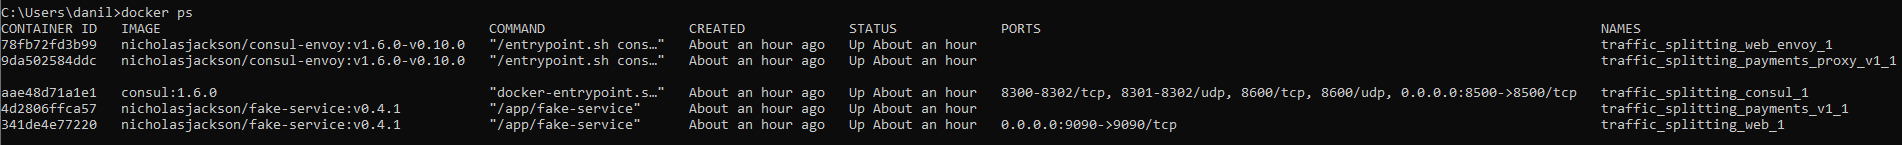
\includegraphics[width=0.9\textwidth]{consul_services_deployment}
    \caption{Deployovani kontejneri}
    \label{fig:consul-services-deployment}
\end{figure} 

Consul automatski radi detekciju servisa i automatske health check-ove prilikom registracije. Prikaz service-discovery-ja je dat na slici \ref{fig:consul-service-discovery}. Na slici vidimo da se uz ime svakog od servisa vidi i zeleni štrik koji ukazuje da je svaki od servisa prošao sve health check-ove. \newline

\begin{figure}[h]
    \centering
    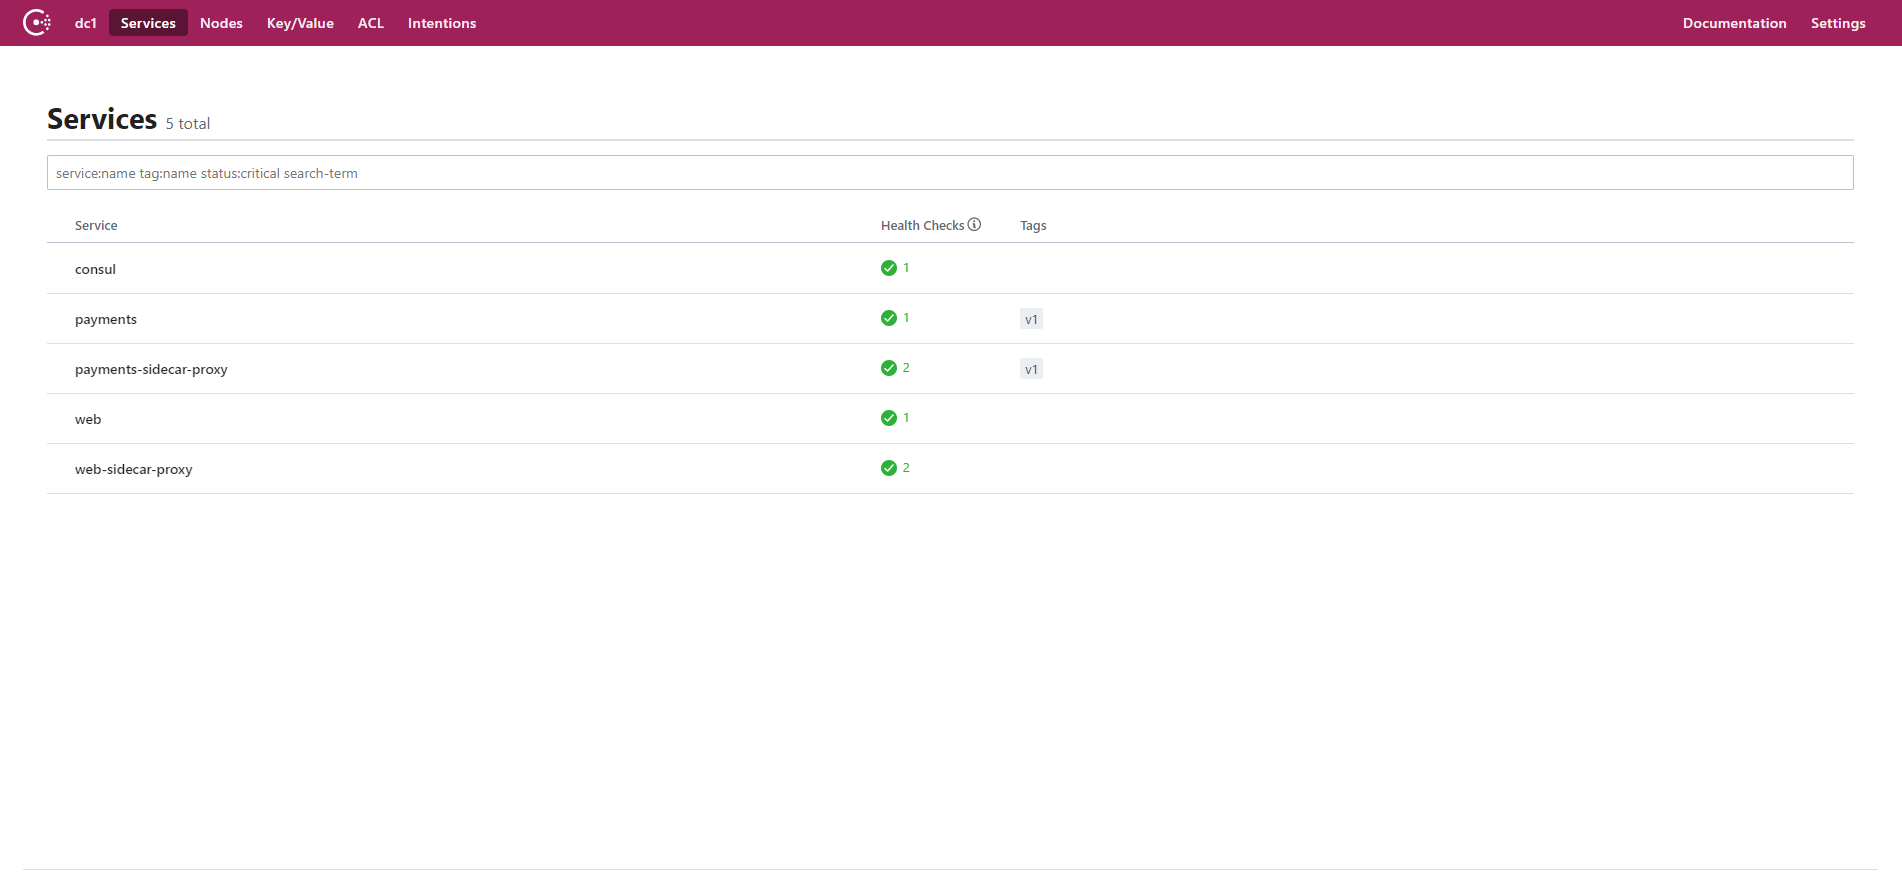
\includegraphics[width=0.9\textwidth]{consul_service_discovery}
    \caption{Consul service discovery}
    \label{fig:consul-service-discovery}
\end{figure} 

Svaki od servisa koje Consul treba da registeruje prolaze kroz 1 health check, tzv node health check, da se vidi da li se može pogoditi host servisa i da li odgovara. Proxy-ji prolaze kroz jedan dodatni service health check i njime se  utvrđuje da li je TCP port koji je naveden u konfiguraciji otvoren i da li može da odgovori na zahteve. Na slici \ref{fig:service-health-check} je dat prikaz health check-a kroz koji je prošao payments servis. Na slici \ref{fig:proxy-health-check} je dat prikaz health check-ova kroz koje je prošao payments proxy. \newline

\begin{figure}[h]
    \centering
    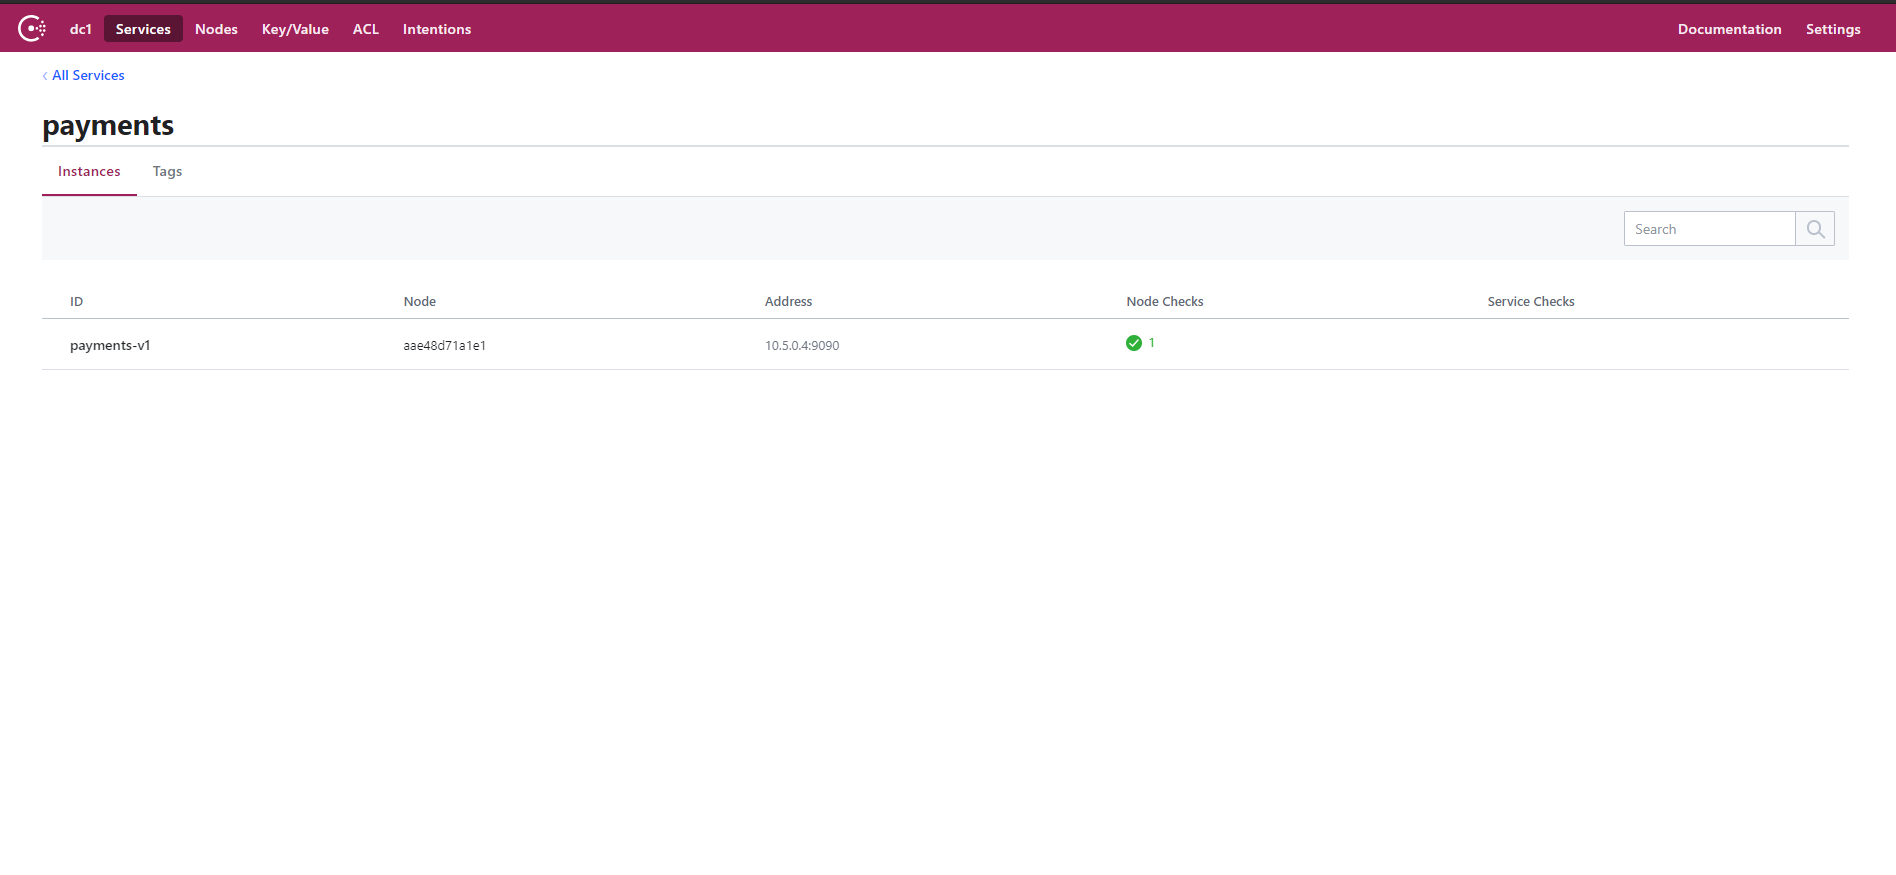
\includegraphics[width=0.9\textwidth]{service_health_check}
    \caption{Payment servis health checks}
    \label{fig:service-health-check}
\end{figure} 

\begin{figure}[h]
    \centering
    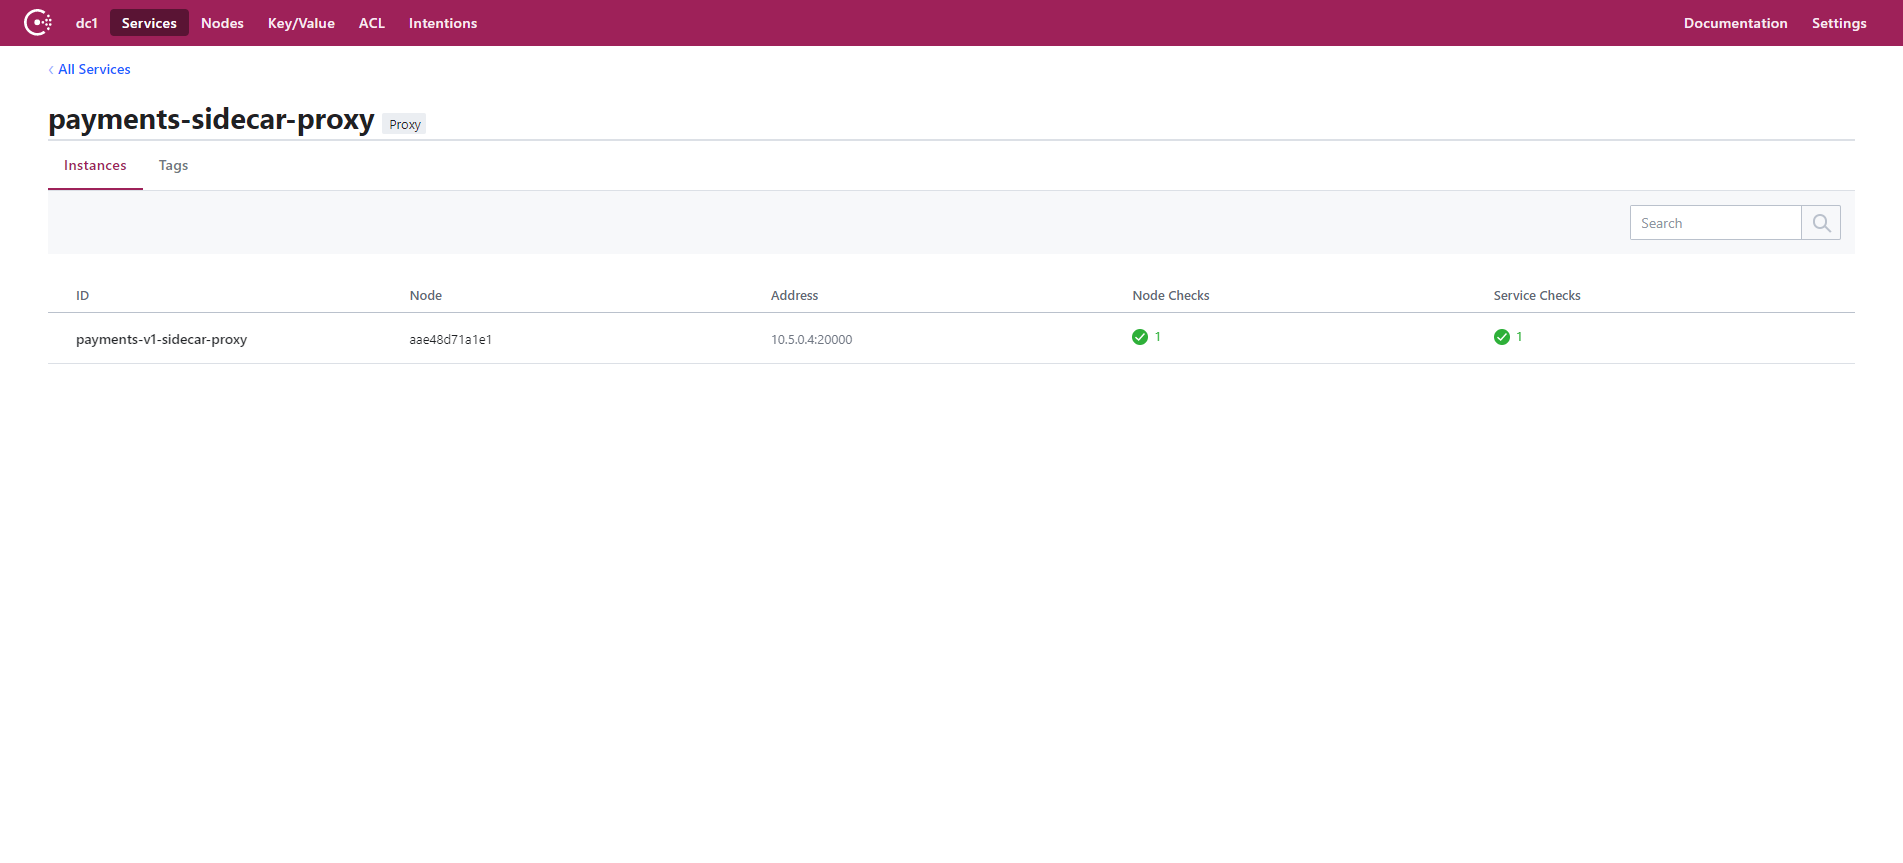
\includegraphics[width=0.9\textwidth]{proxy_health_check}
    \caption{Payment proxy health checks}
    \label{fig:proxy-health-check}
\end{figure}

Ako pošaljemo zahtev GET na localhost:9090, dobićemo odgovor od payment servisa koji se očekuje i koji je dat na slici \ref{response-payments-v1}. \newline

\begin{lstlisting}[
    basicstyle=\small,
    caption = Odgovor na HTTP GET zahtev na adresi localhost:9090, 
   label = response-payments-v1
]
{
  "name": "web",
  "type": "HTTP",
  "duration": "22.4807ms",
  "body": "Hello World",
  "upstream_calls": [
    {
      "name": "payments-v1",
      "uri": "http://localhost:9091",
      "type": "HTTP",
      "duration": "35.9ms",
      "body": "PAYMENTS V1"
    }
  ]
}
\end{lstlisting}

Consul automatski vrši load balancing bez uplitanja korisnika, između više instanci istog servisa. \newline

Zahvaljujući brojnim opcijama konfiguirisanja rutiranja, kod Consula je prilično jednostavno izvesti A/B testiranje i Canary release. Potrebno je da se uvede verzija 2 payments servisa u sistem. Strukturni dijagram aplikacije nakon uvođenja novog servisa dat je na slici \ref{fig:structure-diagram-v2}. \newline

\begin{figure}[h]
    \centering
    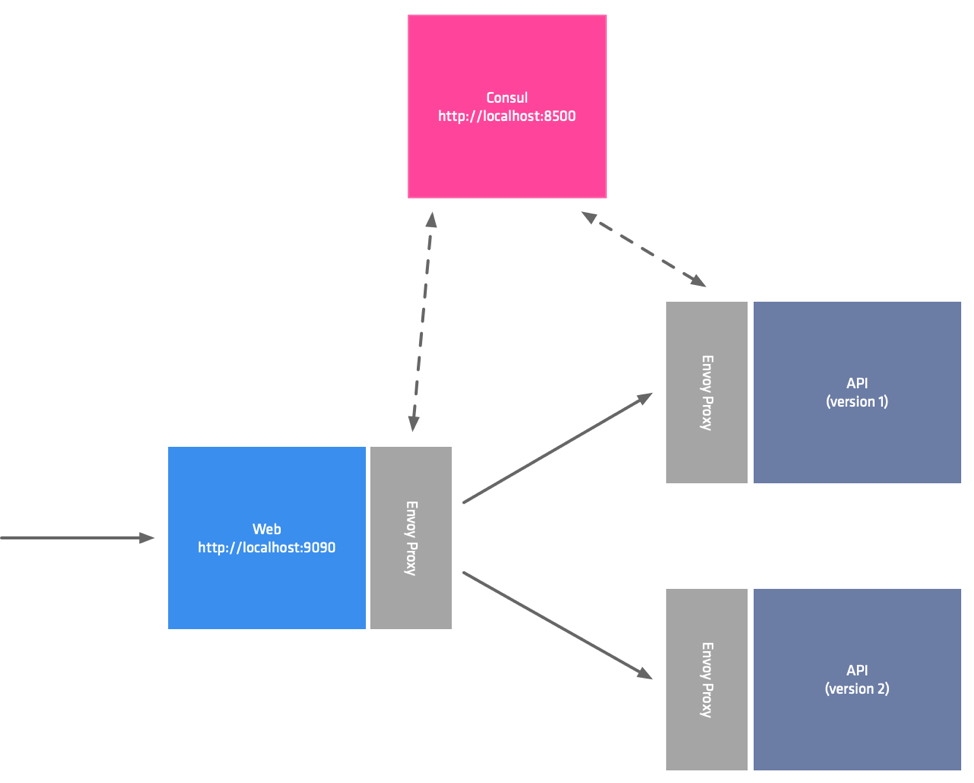
\includegraphics[width=0.9\textwidth]{app_structure_diagram}
    \caption{Strukturni dijagram aplikacije sa dodatim servisom}
    \label{fig:structure-diagram-v2}
\end{figure} 

Pre nego što se deploy-a payment servis v2, potrebno je konfigurisati traffic splitting. Da bi se omogućilo to razdvajanje saobraćaja potrebno je da se primene 3 konfiguraciona fajla: 

\begin{itemize}
	\item Service defaults
	\item Service splitter 
	\item Service resolver
\end{itemize}

\textbf{Konfigurisanje service defaults}\newline

Razdvajanje saobraćaja zahteva da i upstream aplikacije koriste HTTP protokol, jer se razdvajanje dešava na 7 OSI sloju (za svaki zahtev zasebno). Potrebno je naglasiti Consulu da i upstream servisi koriste HTTP tako što se u service defaults naglasi to. Primer ovog konfiguracionog fajla nalazi se na slici \ref{service-defaults}. Polje kind naglašava tip konfiguracije koja se definiše, u ovom slučaju to je service-defaults. Polje name definiše servis na koji se odnosi service-defaults konfiguracija. Polje protokol označava protokol koji se definiše i u ovom slučaju je to HTTP. \newline

\begin{lstlisting}[
    basicstyle=\small,
    caption = Service defaults konfiguracija, 
   label = service-defaults
]
{
  "kind": "service-defaults",
  "name": "api",
  "protocol": "http"
}
\end{lstlisting}

Da bi promene iz konfiguracionog fajla bile primenjene, potrebno je poslati fajl sa slike  \ref{service-defaults} na adresu \texttt{http://localhost:8500/v1/config}, korišćenjem PUT zahteva. \newline

\textbf{Konfigurisanje Service Resolvera}\newline

Sledeće što treba konfigurisati je service resolver opcija. Service resolver omogućava da se podesi kako se biraju instance servisa za neko ime servisa. Service reslover omogućava da se filtrira podskup sevisa na osnovu informacija koje su pružene u trenutku registracije. U ovom slučaju, smo payment servis registrovali sa određenim metapodacima koji su vidljivi na \ref{payments-service-conf}. Vidi se da je payments servis na početku bio registrovan sa tagom v1 i meta verzijom 1. Potrebno je da kreiramo dva podskupa na osnovu ovih podataka (tag i meta verzija). Zato nam služi service-resolver. Svi servisi koji imaju meta verziju 1 i tag v1, biće smešteni u jedan podskup, svi servisi koji imaju tag v2 i meta verziju 2, biće smešteni u drugi podskup. Na slici je prikazana konfiguracije service resolver-a. Takođe, da bi promene iz konfiguracionog fajla bile primenjene, potrebno je poslati fajl sa slike  \ref{service-resolver} na adresu \texttt{http://localhost:8500/v1/config}, korišćenjem PUT zahteva. \newline

\begin{lstlisting}[
    basicstyle=\small,
    caption = Service resolver konfiguracija, 
   label = service-resolver
]
{
  "kind": "service-resolver",
  "name": "api",

  "subsets": {
    "v1": {
      "filter": "Service.Meta.version == 1"
    },
    "v2": {
      "filter": "Service.Meta.version == 2"
    }
  }
}
\end{lstlisting}

\textbf{Konfigurisanje Service splittinga}\newline

Poslednja konfiguracija koju treba primeniti se odnosi na procenat saobraćaja koji će biti prosleđen jednom i drugom podskupu servisa. Inicijalno, treba 100\% saobraćaja da bude usmereno na podskup v1. Konfiguracioni fajl kojim se ovo omogućava dat je na slici \ref{service-splitting-1}. Takođe je i njega potrebno primeniti na adresu \texttt{http://localhost:8500/v1/config}, korišćenjem PUT zahteva. \newline

\begin{lstlisting}[
    basicstyle=\small,
    caption = Service splitting konfiguracija, 
   label = service-splitting-1
]
{
  "kind": "service-splitter",
  "name": "api",
  "splits": [
    {
      "weight": 100,
      "service_subset": "v1"
    },
    {
      "weight": 0,
      "service_subset": "v2"
    }
  ]
}
\end{lstlisting}

Posle ovoga, verzija 2 payment servisa se može deploy-ovati na server. Kako bi se i ova verzija aplikacije deploy-ovala i to u istu mrežu sa ostalim servisima potrebno je da se za nju kreira poseban docker-compose fajl. Deo docker-compose fajla koji se odnosi na verziju 2 payments servisa dat je na slici \ref{payments-v2-dc}. Uz sam servis se deploy-a i odgovarajući proxy. \newline

\begin{lstlisting}[
    basicstyle=\small,
    caption = Deo docker-compose fajla koji se odnosi na payments servis verziju 2, 
   label = payments-v2-dc
]
  payments_v2:
    image: nicholasjackson/fake-service:v0.4.1
    environment:
      UPSTREAM_URIS: http://localhost:9091
      LISTEN_ADDR: localhost:9090
      NAME: payments-v2
      MESSAGE: "PAYMENTS V2"
    networks:
      vpcbr:
        ipv4_address: 10.5.0.6
  payments_proxy_v2:
    image: nicholasjackson/consul-envoy:v1.6.0-v0.10.0
    environment:
      CONSUL_HTTP_ADDR: 10.5.0.2:8500
      CONSUL_GRPC_ADDR: 10.5.0.2:8502
      SERVICE_CONFIG: /config/payments_v2.hcl
      #  CENTRAL_CONFIG: "/central_config/api_service_resolver.hcl;/central_config/api_service_splitter_100_0.hcl"
    volumes:
      - "./service_config:/config"
      - "./central_config:/central_config"
    command: ["consul", "connect", "envoy","-sidecar-for", "payments-v2"]
    network_mode: "service:payments_v2"

\end{lstlisting}

Na slici \ref{fig:payment-sd} je dat prikaz dve različite instance payment servisa - v1 i v2, kako ih Consul vidi. \newline
 
\begin{figure}[h]
    \centering
    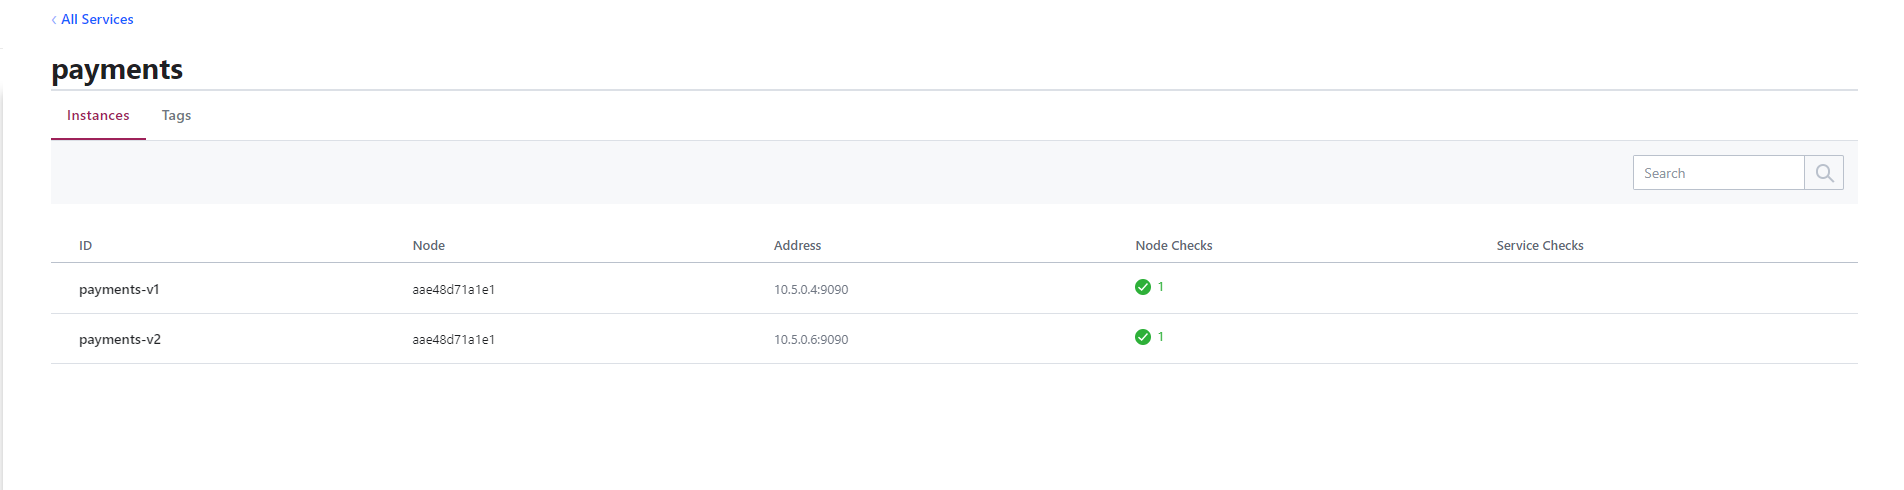
\includegraphics[width=0.9\textwidth]{payment_service_discovery_v1_v2}
    \caption{Payment servis sa dve različite instance}
    \label{fig:payment-sd}
\end{figure} 

Nakon uspešnog deploymenta, potrebno je da sada podesimo Consul da saobraćaj deli 50-između dve različite grupe servisa. To se postiže slanjem novog service-splitter fajla koji je dat na slici \ref{service-splitting-2}.  \newline 
\begin{lstlisting}[
    basicstyle=\small,
    caption = Service splitting konfiguracija 50-50, 
   label = service-splitting-2
]
{
  "kind": "service-splitter",
  "name": "api",
  "splits": [
    {
      "weight": 50,
      "service_subset": "v1"
    },
    {
      "weight": 50,
      "service_subset": "v2"
    }
  ]
}
\end{lstlisting}

Odgovori koji se dobijaju slanjem GET zahteva na localhost:9090 treba da variraju, u odnosu 50-50, između onog datog na slici \ref{response-payments-v1} i slici \ref{response-payments-v2}. Na kraju, sav saobraćaj je potrebno preusmeriti ka payment servisu, v2 da bi Canary release bio uspešno izvršen. Na slici \ref{service-splitting-3} na kojoj je prikazan konfiguracioni fajl kojim se ovo postiže. \newline

\begin{lstlisting}[
    basicstyle=\small,
    caption = Response od payment servisa v2, 
   label = response-payments-v2
]
  "name": "web",
  "type": "HTTP",
  "duration": "54.1339ms",
  "body": "Hello World",
  "upstream_calls": [
    {
      "name": "payments-v2",
      "uri": "http://localhost:9091",
      "type": "HTTP",
      "duration": "28.7891ms",
      "body": "PAYMENTS V2",
      "upstream_calls": [
        {
          "name": "currency",
          "uri": "http://localhost:9091",
          "type": "HTTP",
          "duration": "30.2ms",
          "body": "2 USD for 1 GBP"
        }
      ]
    }
  ]
}
\end{lstlisting}

\begin{lstlisting}[
    basicstyle=\small,
    caption = Service splitting konfiguracija 0-100, 
   label = service-splitting-3
]
{
  "kind": "service-splitter",
  "name": "api",
  "splits": [
    {
      "weight": 0,
      "service_subset": "v1"
    },
    {
      "weight": 100,
      "service_subset": "v2"
    }
  ]
}
\end{lstlisting}

\subsubsection{Rutiranje}

Consul ima podršku za rutiranje zahteva. U odnosu na resurs koji je se gađa, Consul može da rutira zahtev ka odgovarajućem servisu. Uz deployment payment servisa (slika \ref{payments-service-dc}) i Consul servera (slika \ref{dc-consul} ), potrebno je i instancirati novi servis, currency servis. Na slici \ref{currency-ds} je dat deo docker-compose fajla koji se odnosi na currency servis i njegov proxy. \newline 

\begin{lstlisting}[
    basicstyle=\small,
    caption = Deo docker-compose fajla koji se odnosi na Currency servis, 
   label = currency-ds
]
  currency:
    image: nicholasjackson/fake-service:v0.4.1
    environment:
      LISTEN_ADDR: localhost:9090
      NAME: currency
      MESSAGE: "Currency"
      SERVER_TYPE: "http"
    networks:
      vpcbr:
        ipv4_address: 10.5.0.5
  currency_proxy:
    image: nicholasjackson/consul-envoy:v1.6.0-v0.10.0
    environment:
      CONSUL_HTTP_ADDR: 10.5.0.2:8500
      CONSUL_GRPC_ADDR: 10.5.0.2:8502
      SERVICE_CONFIG: /config/currency_v1.hcl
    volumes:
      - "./service_config:/config"
    command: ["consul", "connect", "envoy","-sidecar-for", "currency-v1"]
    network_mode: "service:currency"
\end{lstlisting}

Nakon deploymenta, potrebno je da se naglasi Consulu da svi zahtevi HTTP GET localhost:9090/currency, treba da se prosledi currency servisu, dok se svi ostali zahtevi treba da se proslede ka payment servisu. Najpre je potrebno da se naglasi Consulu da payment servis i currency servis koriste HTTP protokol, i to se radi podesavanjem service-defaults opcije. Na slici \ref{currency-service-defaults} je dato podešavanje service-defaults za currency servis, a na slici \ref{payments-service-defaults} za payments servis. Oba ova podešavanja je potrebno poslati na adresu \texttt{http://localhost:8500/v1/config}, korišćenjem PUT zahteva \newline

\begin{lstlisting}[
    basicstyle=\small,
    caption = Service defaults podesavanje za currency servis, 
   label = currency-service-defaults
]
{
  "kind": "service-defaults",
  "name": "currency",
  "protocol": "http"
}
\end{lstlisting}

\begin{lstlisting}[
    basicstyle=\small,
    caption = Service defaults podesavanje za payments servis, 
   label = payments-service-defaults
]
{
  "kind": "service-defaults",
  "name": "payments",
  "protocol": "http"
}
\end{lstlisting}

Zatim je potrebno da se prosledi service-router podešavanje za payment servis ka Consul-u. Ovim se naglašava da svaki zahtev koji ide ka /currency endpointu, treba da se prosledi currency servisu, a svi ostali zahtevi treba da se proslede ka payments servisu. Na slici \ref{payments-service-router} je data konfiguracija koju potrebno poslati na adresu \texttt{http://localhost:8500/v1/config}, korišćenjem PUT zahteva \newline

\begin{lstlisting}[
    basicstyle=\small,
    caption = Service router podešavanja za Consul rutiranje, 
   label = payments-service-router
]
{
    "kind": "service-router",
    "name": "payments",
    "routes": [
        {
            "match": {
                "http": {
                    "path_prefix": "/currency"
                }
            },
            "destination": {
                "service": "currency"
            }
        },
        {
            "match": {
                "http": {
                    "path_prefix": "/"
                }
            },
            "destination": {
                "service": "payments"
            }
        }
    ]
}
\end{lstlisting}

Nakon uspešne primene podešavanja, ako pošaljemo HTTP GET na localhost:9090/currency dobićemo odgovor kao na slici \ref{currency-response}. U suprotnom, ako se pošalje zahtev na localhost:9090, dobija se odgovor kao na slici \ref{payments-response}. 

\begin{lstlisting}[
    basicstyle=\small,
    caption = Odgovor na /currency, 
   label = currency-response
]
{
  "name": "web",
  "type": "HTTP",
  "duration": "30.2717ms",
  "body": "Hello World",
  "upstream_calls": [
    {
      "name": "currency",
      "uri": "http://localhost:9091",
      "type": "HTTP",
      "duration": "31.9ms",
      "body": "2 USD for 1 GBP"
    }
  ]
}
\end{lstlisting}

\begin{lstlisting}[
    basicstyle=\small,
    caption = Odgovor na /, 
   label = payments-response
]
{
  "name": "web",
  "type": "HTTP",
  "duration": "14.2487ms",
  "body": "Hello World",
  "upstream_calls": [
    {
      "name": "payments-v1",
      "uri": "http://localhost:9091",
      "type": "HTTP",
      "duration": "31.9ms",
      "body": "PAYMENTS V1"
    }
  ]
}
\end{lstlisting}

\chapter{Zaključak}

Mikroservisna arhitektura ima određene nedostatke u pogledu load balancing-a, skaliranja arhitekture, interservisne komunikacije itd. Svi ovi nedostaci mogu u realnim situacijama da izazovu gubitke podataka, da uzrokuju u većem downtime-u sistema itd. Na više načina je pokušano da se nađe rešenje za ove probleme. Pokušali su ljudi da menjaju servise same po sebi, tako da oni kada šalju poruke obezbeđuju redundansu u slanju, da se implementaira posebna service discovery komponenta, koja bi sama vršila load balancing itd. Drugi pristup je bio infrastrukturni. Ideja je bila da servisi samo implementiraju potrebne biznis funkcionalnosti, a sama infrastruktura na koju su postavljeni će se postarati za sve ostalo. \newline

Najpre se došlo na ideju Enterprise service bus (ESB) komponente. Svi servisi se povezuju na magistralu. Ta magistrala u sebi ima mehanizme za prosleđivanje poruka, za transakcije koje obuhvataju više servisa, za load balancing itd. Dobre strane tog sistema su te što se po prvi put razdvajaju funkcionalnosti servisa, te servis brine o biznis logici, a bus brine o greškama koje se dešavaju. Integracija servisa je bila jednostavna i postojao je način da se povežu različiti servisi, jednostavnom konfiguracijom magistrale. Međutim taj sistem se pokazao kao jako spor i težak za održavanje. Takođe je imao veliku manu, da ako prestane sa radom, ceo sistem je nefunkcionalan. \newline

Kao sledeće rešenje, smišljena je service mesh arhitektura. Kod ovog arhitekturnog obrasca logička podela se svodi na kontrolu ravan i ravan podataka. Kontrolna ravan upravlja globalnom konfiguracijom i distribuira je na ravan podataka. Ravan podataka se sastoji od servisa i proxy-ja, koji zajedno čine sidecar obrazac. Ravan podataka čita konfiguraciju od kontrolne ravni i prema tome upravlja komunikacijom između servisa, prikuplja metriku i brine o bezbednosti sistema. Prednosti service mesh arhitekture su te što ne postoji single-point-of-failure u sistemu, prosto sistem funkcioniše šta god da prestane da radi. Servisi brinu samo o biznis logici, bez uplitanja u bilo šta drugo. Upravljanje sistemom je konfigurabilno, i zahvaljući dobro napisanim proxy-jima, komunikacija u sistemu je brza, bezbedna i efikasna. \newline


\end{document}